\documentclass[pdflatex,sn-mathphys-num,iicol]{sn-jnl}

\usepackage[T1]{fontenc}
\usepackage{amsmath,amssymb}
\usepackage{algorithm}
\usepackage{algpseudocode}
\algrenewcommand\algorithmicrequire{\textbf{Input:}}
\algrenewcommand\algorithmicensure{\textbf{Output:}}
\usepackage{booktabs}
\usepackage{array}
\usepackage{graphicx}
\usepackage{tikz}
\usepackage{pgfplots}
\pgfplotsset{compat=1.17}
\usetikzlibrary{arrows.meta,calc,positioning,patterns}
\hypersetup{hypertexnames=false}
\newcommand{\ci}[3]{\begin{tabular}[c]{@{}c@{}}$#1$\\{}[$#2$, $#3$]\end{tabular}}
\newcommand{\cib}[3]{{\boldmath\ci{#1}{#2}{#3}}}
\newcommand{\cit}[3]{\begin{tabular}[t]{@{}c@{}}$#1$\\{}[$#2$, $#3$]\end{tabular}}
\newcommand{\cibt}[3]{{\boldmath\cit{#1}{#2}{#3}}}
\newcommand{\scl}{SCL}
\newcommand{\aob}{AOB}
\newcommand{\twol}[2]{\begin{tabular}[c]{@{}l@{}}#1\\#2\end{tabular}}

\makeatletter
\def\email#1{\global\advance\emailcnt by 1\relax
\if@corauemail
  \ifx\corrauthemail\@empty\g@addto@macro\corrauthemail{\textcolor{blue}{#1}}%
  \else\g@addto@macro\corrauthemail{;\ \textcolor{blue}{#1}}\fi
\else
  \ifx\authemail\@empty\g@addto@macro\authemail{\textcolor{blue}{#1}}%
  \else\g@addto@macro\authemail{;\ \textcolor{blue}{#1}}\fi
\fi}
\makeatother

\begin{document}

\title[Self-Calibrating Control Layer for Multi-Object Trackers]{Training-Free Self-Calibrating Control Layer for Heterogeneous Multi-Object Trackers}

\author*[1]{\fnm{Ahmed Gouda} \sur{Ismail}}\email{a7medgouda1@gmail.com}
\author[1]{\fnm{Mohamed S.} \sur{Mohamed}}\email{mohamedms@mtc.edu.eg}
\author[2]{\fnm{Tarek Ahmed} \sur{Mahmoud}}\email{tarek.mohamed@eui.edu.eg}

\affil*[1]{\orgdiv{Computer Engineering and Artificial Intelligence Department}, \orgname{Military Technical College}, \orgaddress{\city{Cairo}, \country{Egypt}}}
\affil[2]{\orgdiv{Computer Engineering Department}, \orgname{Egypt University of Informatics}, \orgaddress{\city{Cairo}, \country{Egypt}}}

\abstract{Multi-object tracking systems usually have two parts: a detector, which finds objects in each frame and gives each a confidence score, and a tracker, which links them over time using fixed score thresholds. When the detector is replaced, retrained, or compressed, its scores change, but the tracker keeps thresholds set for the old detector. This paper presents a training-free self-calibrating control layer (\scl{}) placed between an unchanged detector and an unchanged tracker (the host). \scl{} splits the scores of recent frames with Otsu's histogram threshold and decides whether they are clean or noisy. On clean scores it keeps the host's settings; on noisy scores it chooses which detections reach the host, rescores them, and sets its thresholds. It also continues tracks for trackers without such a step. It needs no labels and no future frames. One fixed configuration was tested on seven published trackers, four detection sources, and three datasets. Compared with the tracker alone, it raised the higher order tracking accuracy (HOTA) of two single-stage trackers by 0.9\%: OC-SORT, used during development, and PD-SORT, which was not. When all detector scores were halved, two trackers failed completely; with \scl{}, both recovered at least 97\% of their HOTA on the original scores. With a noisy RT-DETR-L detector, it raised the multiple object tracking accuracy (MOTA) of ByteTrack and BoT-SORT by 12.6\% and 16.3\%. On four trackers that already fit their detections, HOTA changed by less than 0.1\%. \scl{} takes 2.95 ms per frame on an ordinary processor.}

\keywords{Multi-object tracking, Tracking by detection, Detector confidence calibration, Online adaptation, Otsu thresholding, Real-time image processing}

\maketitle

\section{Introduction}\label{sec:intro}

Multi-object tracking (MOT) finds every object of interest in a video, such as
people or cars, and gives each object one identity number (ID) that stays the
same over time. It is used in surveillance, driving, and drone systems
\cite{zhu2022visdrone,wu2022uavsurvey}, and many of these systems must give
results with little delay. Most trackers follow the tracking-by-detection
design \cite{adzemovic2026survey}. First, an object detector, a neural network,
looks at each frame and returns candidate boxes. Each box has a confidence
score between 0 and 1 that says how sure the detector is that the box holds an
object. Then a tracker links the boxes of consecutive frames into tracks, one
track per object \cite{bewley2016sort,zhang2022bytetrack,cao2023ocsort}. The
tracker uses a box only if its score passes a fixed limit, called a threshold.
Table~\ref{tab:terms} explains the main terms of this paper in plain words.

Trackers use their thresholds in one of two ways. A two-stage tracker, such as
ByteTrack, first matches the high-score boxes to its tracks and then uses
lower-score boxes in a second step, only to continue tracks that are still
unmatched \cite{zhang2022bytetrack}. A single-stage tracker, such as OC-SORT,
uses one threshold and ignores every box below it \cite{cao2023ocsort}.

In real systems, the detector and the tracker are rarely built together. A
detector is replaced by a faster model, retrained for a new camera, or made
smaller (quantized) for embedded hardware. The tracker, however, keeps the
thresholds that its authors set for another detector. Detector scores are not
calibrated across models and conditions \cite{kuppers2020detcalib}: the same
object can get a high score from one detector and a much lower score from
another. A new detector therefore usually gives scores on a different scale,
and nothing in the system notices the change.

The effect can be large. In this paper, halving the scores of a published
detector reduces two well-known trackers to 0 higher order tracking accuracy
(HOTA) \cite{luiten2021hota}, the main tracking metric of this paper, because
no detection passes their fixed thresholds (Sect.~\ref{sec:shift}). Retuning
every tracker for every detector needs labels from the new setting, that is,
boxes and identities drawn by people, and a working system usually does not
have them.

Current methods solve only part of this problem. Trackers with adaptive
thresholds change their own thresholds from the detections of each frame, but
each method is built into one tracker
\cite{ma2023adaptivebytetrack,shim2024adaptrack,act2026adaptive}. Score
calibration methods correct the detector scores, but they need labelled data
\cite{kuppers2020detcalib}. Methods that adapt a vision system while it runs
learn or measure their settings for one model
\cite{han2022dynamic,jiang2018chameleon}. What is missing is a component that
needs no training, works outside the tracker, adjusts itself from the
detector's own scores, and leaves the tracker alone when it already fits those
scores.

This paper presents such a component: a self-calibrating control layer
(\scl{}) that sits between a detector and a tracker that are both kept fixed
(frozen). We call the tracker that \scl{} serves the \emph{host}, because
\scl{} sits in front of it and works for it without changing its code. The
host gives \scl{} four numbers from its published settings, which we call the
host contract (Sect.~\ref{sec:contract}). The main idea is simple: the
detector's own scores show whether its output fits the host. \scl{} looks at
the scores of recent frames and checks how clearly they separate confident
objects from clutter, that is, boxes that are not real objects. If the
separation is clear, the host keeps its own settings, and the layer only adds
help that the host lacks, such as a step that continues tracks. If it is not
clear, \scl{} chooses which candidates reach the host, gives them new scores,
and sets the host's thresholds. The novelty is therefore a layer outside the
tracker that needs no labels, uses one fixed configuration for many trackers,
and stays out of the way when the tracker already fits the detector.

\begin{table*}[t]
\caption{Main terms of this paper in plain words.}
\label{tab:terms}
\centering\footnotesize
\setlength{\tabcolsep}{4pt}
\renewcommand{\arraystretch}{1.15}
\begin{tabular}{@{}>{\raggedright\arraybackslash}p{32mm}>{\raggedright\arraybackslash}p{123mm}@{}}
\toprule
Term & Meaning in this paper\\
\midrule
Detector & A neural network that finds objects in one video frame and returns a box for each of them.\\
Candidate (detection) & One box returned by the detector, with a class label (for example, car) and a confidence score.\\
Confidence score & A number between 0 and 1 that says how sure the detector is that the box holds an object. Different detectors use different score scales.\\
Threshold & A fixed score limit. The tracker uses a candidate only if its score is at or above the limit.\\
Tracker & A program that links the candidates of consecutive frames into tracks, one track per object.\\
Track, identity (ID) & The boxes of one object over time, with one ID number that should never change.\\
Sequence & One video of a dataset.\\
Stream & The detector output of one video, frame after frame.\\
Host & The tracker that \scl{} serves. It runs after \scl{} with its own published code and settings, which are never changed.\\
Host contract & Four published settings of the host that \scl{} reads (Sect.~\ref{sec:contract}).\\
Matching and birth thresholds & The score a candidate needs to continue an existing track (matching, also called association), and the score it needs to start a new track (birth).\\
Single-stage, two-stage tracker & A single-stage tracker uses one threshold and ignores every candidate below it. A two-stage tracker also uses low-score candidates in a second step, only to continue existing tracks.\\
Frozen & Kept fixed: not retrained, not retuned, not changed in any way.\\
Labels (ground truth) & Boxes and identities drawn by people. They are used only to measure the results, never by \scl{}.\\
Development data & Data that was looked at while \scl{} was designed.\\
Held-out, predeclared & Data or trackers that were chosen in advance, were not used during the design, and were run once with the frozen \scl{}.\\
Logit & The score written on another scale, $\log\bigl(s/(1-s)\bigr)$, Eq.~\eqref{eq:logit}. It spreads out scores close to 0 and 1.\\
Otsu's method & A standard image-processing rule that picks the threshold that best splits a histogram into two groups \cite{otsu1979}.\\
HOTA, MOTA, IDF1 & Tracking metrics in percent; higher is better (Table~\ref{tab:metrics}). HOTA, the main metric, balances finding the objects and keeping their identities.\\
FP, FN, IDS & False positives (boxes where there is no object), false negatives (missed objects), and identity switches (an object's ID changes). They are counts; lower is better.\\
Paired comparison & The same tracker runs twice on the same sequences and detections, once alone and once with \scl{}.\\
95\% interval, significant & The range of likely values of a difference, found by resampling the test sequences 10,000 times (bootstrap). A difference is called significant when this range does not include zero.\\
\bottomrule
\end{tabular}
\end{table*}


The results are consistent across trackers, detectors, and data. With halved
detector scores, \scl{} restored two trackers from 0 to about 66 HOTA. It
improved every single-stage tracker that was tested, including one that was
not seen during design, and it raised HOTA on every MOT17 sequence for both of
them. With other detectors, it raised the multiple object tracking accuracy
(MOTA), a metric that counts errors, of two-stage trackers by up to 7.9 points
on KITTI and by 24.7 points on held-out aerial data, that is, data that was
not used during the design. On the same scores, it reached higher HOTA than
simple adaptive thresholds by 2.2 to 8.6 points, and it was ahead of the
published adaptive-threshold method ACT under halved scores (by 2.0 and 10.1
HOTA points) and on held-out aerial data (by 1.8 HOTA points with YOLOv8n and
22.7 MOTA points with RT-DETR-L). Strong trackers that already fit their
detector kept their accuracy, and no statistically significant HOTA loss was
found in any tested combination of data, detector, and tracker. The layer
takes about 3 ms per frame on an ordinary processor (central processing unit,
CPU).

The main contributions are:
\begin{enumerate}
\item \scl{}, a control layer that needs no training, adjusts itself from the
      detector scores, uses no future frames, keeps the tracker's settings
      when the scores are clean, and takes full control only when they are
      noisy (Sect.~\ref{sec:method}).
\item A host contract, a set of four numbers from the tracker's published
      settings, that lets one fixed configuration work with single-stage and
      two-stage trackers without changing them (Sect.~\ref{sec:contract}).
\item A development path from always-on banding (\aob{}), an earlier design
      that always intervened, in which each step is compared with that
      design (Sect.~\ref{sec:development}).
\item A test of one fixed configuration on seven published trackers, four
      detection sources, and three datasets: on data used during the design,
      and on trackers and data that were chosen in advance and run only once.
      The test includes statistical intervals for every difference, a
      comparison with simple adaptive thresholds and with the published ACT
      method, an analysis of each part of the layer, and a speed measurement
      on a CPU (Sects.~\ref{sec:setup} and~\ref{sec:results}).
\end{enumerate}

The rest of the paper is organized as follows. Section~\ref{sec:data-eval}
describes the data, the evaluation roles, and the metrics, and
Section~\ref{sec:related} reviews related work. Section~\ref{sec:method}
explains \scl{} and all its settings, and Section~\ref{sec:development} shows
how it was developed from an earlier design that always intervened. The
configuration was then frozen before any external system was run.
Section~\ref{sec:setup} gives the experimental setup,
Section~\ref{sec:results} the results and their analysis, and
Section~\ref{sec:conclusion} concludes the paper.

\section{Data and Evaluation}\label{sec:data-eval}

\subsection{Detectors and data}\label{sec:data}
Table~\ref{tab:data} lists the evaluation cells. A cell is one combination of
data, detector, and tracker (the trackers are introduced in
Sect.~\ref{sec:setup}). Three public datasets are used. MOT17
\cite{milan2016mot16} shows people in city scenes. As is common, each of its
training videos is split in time, and the second half, called val-half, is
used for evaluation. On MOT17 the trackers use the published detections of
the YOLOX-X detector \cite{ge2021yolox}, so every tracker sees exactly the
same boxes. A detector drops the boxes whose score is below a small value
before it passes them on; we call this value the emission floor. The two
published MOT17 detection sets have floors of 0.01 and 0.1
(Sect.~\ref{sec:tracker}). KITTI tracking \cite{geiger2012kitti} shows cars
and pedestrians seen from a driving car. On its training set the trackers run
with two detectors that differ from the MOT17 detector: YOLOv8n
\cite{jocher2023yolov8}, a small and fast model, and RT-DETR-L
\cite{zhao2024rtdetr}, a larger transformer model. UAVDT \cite{du2018uavdt}
shows vehicles seen from drones. Its test split, 20 sequences with 16,592
frames, was not used during the design; ByteTrack runs on it with the same two
detectors, restricted to their vehicle classes.

To study the score problem directly, the published MOT17 scores were also
changed before the tracker by four monotone transforms, which change the
score values but keep their order: cubing ($s^3$), halving ($0.5\,s$), and
logit temperatures $T=2$ and $T=0.5$, $\sigma(z/T)$, where $\sigma$ turns a
logit back into a score. A temperature divides the logit $z$ of each score by
$T$ before turning it back into a score: $T=2$ pulls all scores toward 0.5,
and $T=0.5$ pushes them toward 0 and 1. These transforms imitate the score
changes that a new or retrained detector can cause. The trackers kept their
published thresholds. The external systems use the detections released by
their authors on MOT17 val-half.

\begin{table*}[t]
\caption{Evaluation cells and their role. A cell is one combination of data,
detector, and tracker. Development cells were looked at while the layer was
designed; predeclared and held-out cells were chosen in advance and run once
with the frozen layer.}
\label{tab:data}
\centering\footnotesize
\setlength{\tabcolsep}{4pt}
\begin{tabular}{@{}>{\raggedright\arraybackslash}p{29mm}>{\raggedright\arraybackslash}p{25mm}>{\raggedright\arraybackslash}p{42mm}>{\raggedright\arraybackslash}p{25mm}@{}}
\toprule
Data & Detector & Trackers & Role\\
\midrule
MOT17 val-half (7 sequences) & published YOLOX-X detections & ByteTrack (2 settings), OC-SORT, BoostTrack, SparseTrack & development\\
KITTI tracking training (21 sequences) & RT-DETR-L; YOLOv8n & ByteTrack and BoT-SORT (RT-DETR-L); OC-SORT (YOLOv8n) & development (detector transfer)\\
MOT17 val-half, score transforms & published YOLOX-X, transformed scores & ByteTrack (2 settings), OC-SORT, BoostTrack & development (robustness)\\
MOT17 val-half & released PD-SORT / Hybrid-SORT detections & PD-SORT, Hybrid-SORT & predeclared external\\
UAVDT test (20 sequences) & RT-DETR-L; YOLOv8n & ByteTrack & predeclared held-out\\
KITTI tracking training, also with halved scores & RT-DETR-L; YOLOv8n & ByteTrack (RT-DETR-L); OC-SORT (YOLOv8n) & development (baselines, ACT, and components)\\
\bottomrule
\end{tabular}
\end{table*}


\subsection{Evaluation roles and metrics}\label{sec:roles}
Every cell has one of two roles (Table~\ref{tab:data}). Development cells
were looked at while \scl{} was designed: MOT17 with four trackers, KITTI
with two other detectors, and the score transforms. The other cells test
\scl{} on trackers and data that it had never seen. The two predeclared
external trackers, PD-SORT and Hybrid-SORT, were chosen and named before they
were run, and they were run once with the frozen configuration. The held-out
UAVDT test split was also run once with the frozen configuration, after a
written plan. To check that each external tracker was run correctly, our run
of the tracker alone is compared with the number reported by its authors and
marked EXACT (within 0.2 HOTA points) or CLOSE (within 1.0 HOTA point, with a
known cause that was not tuned).

\label{sec:metrics}Table~\ref{tab:metrics} gives the tracking metrics and
their definitions. They are built from four counts: false positives (FP),
boxes where there is no object; false negatives (FN), objects that were
missed; identity switches (IDS), cases where an object's ID changes; and the
number of ground-truth boxes (GT). HOTA is the main metric, because it
balances finding the objects and keeping their identities. MOTA counts errors
and reacts mostly to FP and FN, and the identity F1 score (IDF1) measures how
long each object keeps its correct ID. IDS should be read together with FN: a
tracker that follows more objects has more chances to switch identities, so
IDS can rise while the tracking as a whole becomes better. The metrics are
computed with the TrackEval library (commit 12c8791) and the official ground
truth of each benchmark, following MOTChallenge practice
\cite{dendorfer2021motchallenge}. On KITTI tracking, HOTA is the official
value averaged over cars and pedestrians. On UAVDT, all vehicles form one
class, and predictions inside the regions that the dataset marks as ignored
are removed.

\begin{table*}[t]
\caption{Tracking metrics used in this paper. GT is the number of
ground-truth boxes; FP, FN, and IDS are the false positives, missed objects
(false negatives), and identity switches, summed over all frames. For IDF1,
each ground-truth track is first matched to at most one output track, and
IDTP, IDFP, and IDFN are the true-positive, false-positive, and
false-negative boxes under this matching. For HOTA, at a localization
threshold $\alpha$, $\mathrm{TP}_\alpha$, $\mathrm{FN}_\alpha$, and
$\mathrm{FP}_\alpha$ are the matched, missed, and unmatched boxes, and
$\mathcal{A}(c)$ is the association accuracy of a matched pair $c$. HOTA,
MOTA, and IDF1 are given in percent.}
\label{tab:metrics}
\centering\footnotesize
\setlength{\tabcolsep}{4pt}
\renewcommand{\arraystretch}{1.6}
\begin{tabular}{@{}l>{\raggedright\arraybackslash}p{64mm}>{\raggedright\arraybackslash}p{46mm}@{}}
\toprule
Metric & Definition & What it measures\\
\midrule
FP, FN, IDS & counts summed over all frames & FP: boxes where there is no object; FN: objects that were missed; IDS: times an object's ID changes. Lower is better; IDS is read together with FN, because a tracker that follows more objects has more chances to switch IDs\\
MOTA \cite{bernardin2008clear} & $\displaystyle \mathrm{MOTA}=1-\frac{\mathrm{FN}+\mathrm{FP}+\mathrm{IDS}}{\mathrm{GT}}$ & one minus the share of errors; reacts mostly to false positives and missed objects\\
IDF1 \cite{ristani2016idf1} & $\displaystyle \mathrm{IDF1}=\frac{2\,\mathrm{IDTP}}{2\,\mathrm{IDTP}+\mathrm{IDFP}+\mathrm{IDFN}}$ & how long each object keeps its correct ID\\
HOTA \cite{luiten2021hota} & $\displaystyle \mathrm{HOTA}=\frac{1}{19}\sum_{\alpha}\sqrt{\mathrm{DetA}_\alpha\,\mathrm{AssA}_\alpha}$,\newline $\displaystyle \mathrm{DetA}_\alpha=\frac{|\mathrm{TP}_\alpha|}{|\mathrm{TP}_\alpha|+|\mathrm{FN}_\alpha|+|\mathrm{FP}_\alpha|}$,\quad $\displaystyle \mathrm{AssA}_\alpha=\frac{1}{|\mathrm{TP}_\alpha|}\sum_{c\in\mathrm{TP}_\alpha}\mathcal{A}(c)$,\newline with $\alpha=0.05,0.10,\dots,0.95$ & balance of finding the objects (detection accuracy, DetA) and keeping their identities (association accuracy, AssA); the main metric of this paper\\
\bottomrule
\end{tabular}
\end{table*}


All comparisons are paired: each tracker runs twice on the same sequences and
detections, once alone and once with \scl{}, and nothing else changes. The
difference is computed over all sequences together. To show how
certain a difference is, we use a bootstrap \cite{efron1993bootstrap}: the
sequences are drawn again at random, with repetition, 10,000 times (with the
fixed random seed 42, so that the result can be repeated),
the difference is computed again each time, and the middle 95\% of these
values gives the 95\% interval. A difference is called significant when its
interval does not include zero; bold intervals in the tables mark such
differences. As a simple check that needs no statistics, we also count the
sequences where HOTA rose, stayed the same ($|\Delta\mathrm{HOTA}|<0.01$), or
fell.

HOTA, MOTA, and IDF1 are given in percent, and higher values are better. FP,
FN, and IDS are counts, and lower values are better. Runtime is given in
milliseconds (ms) per frame, and lower values are better.

\section{Related Work}\label{sec:related}

\scl{} is related to four lines of research: the trackers it works with, the
confidence of the detectors that feed them, trackers that adapt their own
thresholds, and methods that adapt inference while running. They are
reviewed below in this order, and Table~\ref{tab:related} compares the
closest methods with \scl{}.

Most practical trackers follow the tracking-by-detection design. SORT
predicts where each tracked box will be in the next frame with a Kalman
filter, a standard motion predictor, and matches these predictions to the new
detections by their overlap, using the Hungarian method, which finds the best
one-to-one matching \cite{bewley2016sort}.
ByteTrack added a second matching step that uses low-score detections to
continue existing tracks \cite{zhang2022bytetrack}, and many later trackers
kept this two-stage design. Others, such as OC-SORT \cite{cao2023ocsort}, use
only one score threshold. All these trackers read detector scores through
fixed thresholds that were tuned for one detector, usually YOLOX
\cite{ge2021yolox}. Seven published trackers of both kinds are used in this
paper as hosts, that is, as the trackers that \scl{} serves, and they are not
changed (Sect.~\ref{sec:setup}). A recent survey
groups the tracking-by-detection methods into joint detection and embedding,
heuristic, motion-based, affinity-learning, and offline methods, and compares
them across benchmarks \cite{adzemovic2026survey}.

Many recent trackers improve their association with parts that are trained or
designed for a domain: small re-identification networks, which compare the
appearance of objects \cite{li2024fdbtrack}, learnable graph matching
\cite{bao2024graphmatching,zhang2025sinkhorn}, result-guided feature
extraction for faster tracking \cite{ding2025remot}, motion models for
low-frame-rate surface-vehicle videos \cite{liang2024motiontrack}, and image
restoration by blind super-resolution before tracking in adverse weather
\cite{sun2026bsr}. These methods change or retrain the tracker; \scl{} keeps
both the tracker and the detector unchanged and acts only on what passes
between them.

These fixed thresholds are a weak point, because scores do not mean the same
thing for every detector. Detectors of different families, such as YOLOX
\cite{ge2021yolox}, YOLOv8 \cite{jocher2023yolov8}, YOLOv9
\cite{wang2024yolov9}, DETR \cite{carion2020detr}, and RT-DETR
\cite{zhao2024rtdetr}, give different score distributions. Their confidence
is not calibrated across models and conditions, and calibration methods for
object detection learn a mapping from labelled data
\cite{kuppers2020detcalib}. A tracker tuned for one detector therefore cannot
assume that another detector's scores mean the same thing, and labels to
recalibrate them are rarely available after deployment. Image processing
offers a tool that needs no labels: Otsu's method picks a threshold from a
histogram so that the two resulting groups are as separate as possible
\cite{otsu1979}. \scl{} applies it to the logits (log-odds) of the detector
scores of recent frames.

Some trackers already adapt their own thresholds. Adaptive ByteTrack sets the
score threshold of ByteTrack from the detections of each frame
\cite{ma2023adaptivebytetrack}. AdapTrack adapts the thresholds of its
matching step \cite{shim2024adaptrack}. ACT sets the high and low thresholds
of each frame from the first quartile of the scores and the number of
candidates \cite{act2026adaptive}. Other recent trackers use the score or the
spread of each detection inside the tracker. ConfTrack weights the Kalman
update, the Kalman noise, and the matching cost by the score of each box
\cite{jung2024conftrack}. UTrack measures the spread of the boxes that
non-maximum suppression (NMS), the detector step that removes overlapping boxes
of the same object, merges, and uses it as the Kalman noise, so it needs the
boxes before this step \cite{solano2025utrack}. PlugTrack blends the Kalman
filter with learned motion predictors through a small network trained with
labels \cite{kim2026plugtrack}. These methods are built into the tracker, use
only the current frame or each box alone, or need extra trained parts or the
inside of the detector. \scl{} differs in four ways. It uses past
frames. It decides for the whole video whether to act at all, and otherwise
keeps the tracker's own settings. It works through a host contract, four published
settings of each tracker, on several published trackers without changing them. And it is tested as one
frozen configuration under score changes and on external systems.

A wider group of methods adapts inference itself. Dynamic neural networks
adapt their computation to each input \cite{han2022dynamic}, and Chameleon
measures again, from time to time, which settings of a video analysis system
work best \cite{jiang2018chameleon}. These methods learn or measure their
settings for each model. Our earlier work, AC-MOT (a manuscript submitted for publication), is a controller that
needs no training and sets the detector operating point (score threshold,
NMS threshold, and input resolution) while running, from image and track
cues. Such a controller is tied to the detector it was calibrated with,
because a change in the detector's score scale does not change the image.
\scl{} reads the scores instead and acts on the tracker's input and
thresholds.

In summary, current methods either adapt thresholds or use the score of each
box inside one tracker, calibrate scores with labelled data, or learn their
settings for one model. What is missing is a layer that needs no training, adjusts itself
from the detector's own scores, works with many unchanged trackers, and keeps
a well-matched tracker at its own accuracy. \scl{} is designed to fill this
gap. Table~\ref{tab:related} summarizes the differences.

\begin{table*}[t]
\caption{Comparison of \scl{} with recent adaptive methods for tracking (BT: ByteTrack; ReID: re-identification network; NMS: non-maximum suppression).}
\label{tab:related}
\centering\footnotesize
\setlength{\tabcolsep}{3pt}
\begin{tabular}{@{}>{\raggedright\arraybackslash}p{18mm}c>{\raggedright\arraybackslash}p{21mm}>{\raggedright\arraybackslash}p{19mm}>{\raggedright\arraybackslash}p{15mm}>{\raggedright\arraybackslash}p{16mm}>{\raggedright\arraybackslash}p{21mm}@{}}
\toprule
Method & Year & Adapted & Statistics & Extra trained part & Detector input & Where it works\\
\midrule
Adapt.\ BT \cite{ma2023adaptivebytetrack} & 2023 & high/low score split & current frame & none & boxes and scores & inside BT\\
ConfTrack \cite{jung2024conftrack} & 2024 & Kalman update, noise, and cost & score of each box & ReID & boxes and scores & new tracker\\
AdapTrack \cite{shim2024adaptrack} & 2024 & matching thresholds & current frame & ReID & boxes and scores & new tracker\\
UTrack \cite{solano2025utrack} & 2025 & Kalman noise & spread of boxes merged by NMS & none & boxes before NMS & added to existing trackers\\
ACT \cite{act2026adaptive} & 2026 & high and low thresholds & current frame & none & boxes and scores & inside the tracker\\
PlugTrack \cite{kim2026plugtrack} & 2026 & mix of Kalman and learned motion & track boxes & network trained with labels & boxes & added to two learned predictors\\
K{\"u}ppers \cite{kuppers2020detcalib} & 2020 & detector scores & labelled data & calibration map & boxes and scores & detector output\\
Chameleon \cite{jiang2018chameleon} & 2018 & pipeline configuration & profiling & none & whole pipeline & analytics pipeline\\
AC-MOT (ours, submitted) & 2026 & detector operating point & image and track cues & none & sets its settings & before the detector\\
\scl{} (this paper) & -- & candidates, scores, thresholds & past frames, no labels & none & boxes and scores & between detector and seven unchanged trackers\\
\bottomrule
\end{tabular}
\end{table*}


\section{Method}\label{sec:method}

\scl{} is a small step that runs once per frame between the detector and the
tracker (Fig.~\ref{fig:arch}). It does four things. First, it looks at the
detector scores of the last few frames and puts the candidates into three
groups: background, uncertain, and confident (Sect.~\ref{sec:calib}).
Second, it uses these groups to decide whether the detector output is clean
or noisy (Sect.~\ref{sec:regimes}). Third, it acts on this decision: on
clean scores it keeps the tracker's own settings, and on noisy scores it
chooses which candidates reach the tracker, assigns them new scores, and sets
the tracker's thresholds. Fourth, in both cases it can pass a weak candidate
that clearly continues an existing track (Sect.~\ref{sec:rescue}). The
tracker then runs as usual on what it receives. The detector and the tracker
are never changed, and Sect.~\ref{sec:constants} lists every setting of the
layer.

\begin{figure*}[t]
\centering
\resizebox{\textwidth}{!}{%
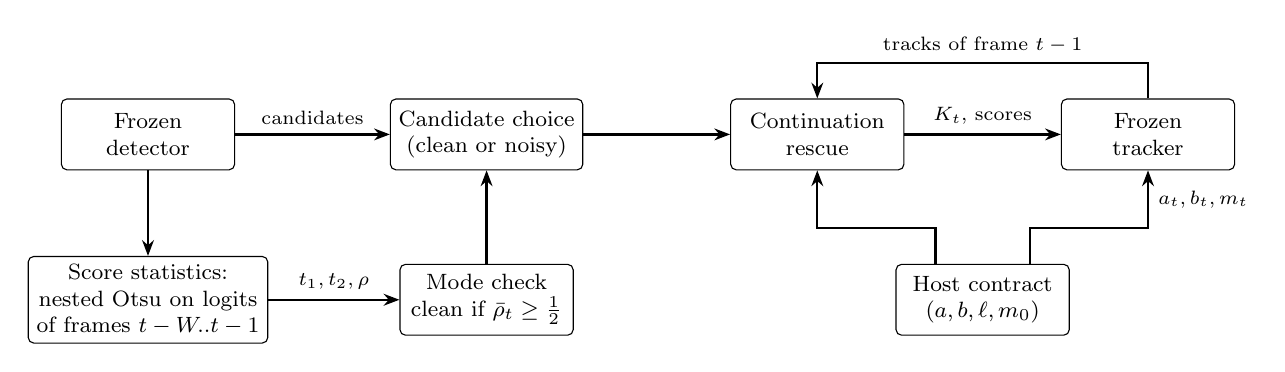
\begin{tikzpicture}[
  box/.style={draw, rounded corners=2pt, align=center, font=\footnotesize, minimum height=9mm, minimum width=22mm, inner sep=3pt},
  arr/.style={-{Stealth[length=2mm]}, thick}, lab/.style={font=\scriptsize}]
\node[box] (det) at (0,0) {Frozen\\detector};
\node[box] (pol) at (4.3,0) {Candidate choice\\(clean or noisy)};
\node[box] (res) at (8.5,0) {Continuation\\rescue};
\node[box] (trk) at (12.7,0) {Frozen\\tracker};
\node[box] (stat) at (0,-2.1) {Score statistics:\\nested Otsu on logits\\of frames $t-W..t-1$};
\node[box] (reg) at (4.3,-2.1) {Mode check\\clean if $\bar\rho_t \ge \tfrac12$};
\node[box] (hc) at (10.6,-2.1) {Host contract\\$(a, b, \ell, m_0)$};
\draw[arr] (det) -- node[lab, above]{candidates} (pol);
\draw[arr] (pol) -- (res);
\draw[arr] (res) -- node[lab, above]{$K_t$, scores} (trk);
\draw[arr] (det) -- (stat);
\draw[arr] (stat) -- node[lab, above]{$t_1, t_2, \rho$} (reg);
\draw[arr] (reg) -- (pol);
\draw[arr] (hc.north) ++(-0.6,0) |- ++(0,0.45) -| (res.south);
\draw[arr] (hc.north) ++(0.6,0) |- ++(0,0.45) -| node[lab, pos=0.75, right]{$a_t, b_t, m_t$} (trk.south);
\draw[arr] (trk.north) -- ++(0,0.45) -| node[lab, pos=0.25, above]{tracks of frame $t-1$} (res.north);
\end{tikzpicture}}
\caption{\scl{} between a frozen detector
and a frozen tracker. The statistics use earlier frames only. The host
contract holds the tracker's published settings. The tracker receives the
chosen candidates, their scores, and its thresholds for the frame}
\label{fig:arch}
\end{figure*}

\subsection{Inputs and outputs}\label{sec:problem}
In each frame $t$, the detector gives a list of candidates
$D_t=\{(\mathbf{x}_i,s_i,c_i)\}$: a box $\mathbf{x}_i$, a score
$s_i\in(0,1)$, and a class label $c_i$ for each one, down to a lowest score
called the emission floor. The layer does not use the score itself but its
logit (log-odds), which spreads out scores close to 0 and 1:
\begin{equation}
z_i=\log\frac{s_i}{1-s_i}.
\label{eq:logit}
\end{equation}
For example, a score of 0.5 gives $z_i=0$, a score of 0.9 gives
$z_i\approx2.2$, and a score of 0.1 gives $z_i\approx-2.2$. The logistic
function $\sigma(z)=1/(1+e^{-z})$ turns a logit back into a score. Table~\ref{tab:symbols}
lists all symbols of the method.

As defined in Sect.~\ref{sec:intro}, the tracker that the layer serves is
called the host. It gives the layer four numbers about itself, the host
contract $h=(a,b,\ell,m_0)$. These are simply the settings that its
authors published: $a$ is the score a detection needs to be matched to a
track in the first step, $b$ is the score it needs to start a new track,
$\ell$ is the lowest score the tracker uses at all, and $m_0$ is its matching
tolerance (one minus the smallest overlap that still counts as a match).
Overlap is measured by the intersection over union (IoU) of two boxes: the
area they share divided by the area they cover together, from 0 (no overlap)
to 1 (the same box). A
single-stage tracker uses one threshold, so $\ell=\min(a,b)$. A two-stage
tracker also uses weaker detections in a second step, so
$\ell<\min(a,b)$.

In every frame the layer returns five things: the candidates $K_t$ that the
tracker will see, their scores $\tilde{s}$, and the thresholds $(a_t,b_t)$
and tolerance $m_t$ that the tracker will use in this frame:
\begin{equation}
\left(K_t,\tilde{s},a_t,b_t,m_t\right)=
\mathcal{L}\left(Z_{<t},D_t,\mathcal{T}_{t-1},g_t;\,h\right).
\label{eq:layer}
\end{equation}
Here $Z_{<t}$ are the logits of the earlier frames, $\mathcal{T}_{t-1}$ are
the tracks of the previous frame, and $g_t$ is an optional measure of camera
motion in frame $t$. In words, Eq.~\eqref{eq:layer} says that the output for
frame $t$ depends only on the logits of earlier frames, the candidates of
frame $t$, the tracks of frame $t-1$, the camera motion, and the tracker's
contract. The decision for frame $t$ uses only past frames; frame $t$ is
added to the statistics after the decision, and no future frame is ever
used.

\begin{table}[t]
\caption{Main symbols of the method.}
\label{tab:symbols}
\centering\footnotesize
\begin{tabular}{@{}l>{\raggedright\arraybackslash}p{51mm}@{}}
\toprule
Symbol & Meaning\\
\midrule
$t$ & frame index\\
$D_t$ & candidates of frame $t$ given by the detector\\
$\mathbf{x}_i, s_i, c_i$ & box, score, and class label of candidate $i$\\
$z_i$ & logit (log-odds) of the score $s_i$, Eq.~\eqref{eq:logit}\\
$\sigma(\cdot)$ & logistic function, turns a logit back into a score\\
$h=(a,b,\ell,m_0)$ & host contract: the tracker's published settings\\
$a$, $b$ & score needed to match a track, and to start a new track\\
$\ell$ & lowest score the tracker uses\\
$m_0$ & matching tolerance: one minus the smallest IoU that counts as a match\\
$W$ & number of past frames used for the statistics (10)\\
$t_1$, $t_2$ & first and second Otsu split on the logits\\
$Z_t^W$ & logits of the last $W$ frames, $t-W$ to $t-1$\\
$\rho_t$, $\bar\rho_t$ & share of confident logits in $Z_t^W$, and the median of all $\rho$ values so far\\
$u_i$ & rank of candidate $i$ among recent scores, from 0 to 1\\
$K_t$, $\tilde{s}$ & candidates passed to the tracker, and their scores\\
$a_t$, $b_t$, $m_t$ & thresholds and tolerance used by the tracker in frame $t$\\
$\mathcal{T}_{t-1}$ & tracks of the previous frame\\
$g_t$, $r_t$ & camera motion in frame $t$, and its ratio to the usual motion\\
IoU & intersection over union: overlap of two boxes, from 0 to 1\\
\bottomrule
\end{tabular}
\end{table}

Four goals guided the design. The layer needs no training and no labels. One
frozen configuration must work for every tracker, detector, and dataset.
When the tracker already fits the detector, its input must stay the same.
And the layer must take little time compared with the detector.

\subsection{Self-calibration from detector scores}\label{sec:calib}
A detector that suits the scene gives many low scores to background and a
separate group of high scores to objects. The layer checks, without labels,
how clearly this happens. It collects the logits of the candidates of the
last $W=10$ frames that remain after duplicate removal
(Sect.~\ref{sec:regimes}) and splits them twice with Otsu's method \cite{otsu1979},
which finds the threshold that best separates a histogram into two groups.
The first split, $t_1$, separates background (low logits) from foreground
(high logits). The second split, $t_2$, is found in the same way on the
foreground logits only, and divides them into uncertain and confident
candidates. We call these two splits nested Otsu splits.
The share of confident candidates in the foreground,
\begin{equation}
\rho_t=\frac{\left|\{z\in Z_t^W: z\ge t_2\}\right|}{\left|\{z\in Z_t^W: z\ge t_1\}\right|},
\label{eq:rho}
\end{equation}
where $Z_t^W$ are the logits of the last $W$ frames, $t-W$ to $t-1$, the same
logits that give $t_1$ and $t_2$. It shows how clearly the detector separates
objects from clutter. In words, $\rho_t$ is the number of confident candidates
divided by the number of foreground candidates in these frames. It is computed
before frame $t$ is processed; the candidates of frame $t$ enter the
statistics only after the decision for frame $t$. For example, if 40 candidates are in the foreground
and 30 of them are confident, then $\rho_t=0.75$. A high $\rho_t$ means that most foreground candidates are confident; a low $\rho_t$
means that many of them are uncertain. Because the splits are made on
logits, they move with the scores when the whole logit scale is stretched or
shifted, for example by a change of temperature, and each group keeps the
same candidates.

These groups only make sense if there is a real background group. Some
detectors give very few low scores; then the first split falls inside the
objects. The layer detects this case, when fewer candidates lie below $t_1$
than above it, and counts the frame as clean, $\rho_t=1$. This background
check covers, for example, the first frames of a sequence with only about
ten candidates per frame, where both splits would otherwise fall among the
objects ($t_1\approx0.6$ and $t_2\approx0.93$ in probability terms).

\subsection{Clean and noisy modes}\label{sec:regimes}
The mode decides how much the layer may change. A clean stream means that
the detector already separates objects from clutter, so the tracker's own
settings are kept. A noisy stream means that many candidates are uncertain,
so the layer takes over the choice of candidates and thresholds.

\emph{Choosing the mode.} The stream is clean at frame $t$ if the median
$\bar\rho_t$ of all $\rho$ values so far (ignoring cold frames) is at least
one half, and noisy otherwise. Before the first valid split, for example in
the first frame, the mode is called cold. Because the median covers the whole
stream so far, the mode describes the detector and the scene, and a short
drop in confidence, for example during fast camera motion, does not change
it.

\emph{Cold and clean modes.} The tracker keeps its own thresholds. In the
clean mode there is one exception: if a threshold is so high that it would
reject the confident group, it is lowered to $t_2$:
\begin{equation}
a_t=\min\!\left(a,\sigma(t_2)\right),\qquad b_t=\min\!\left(b,\sigma(t_2)\right),
\label{eq:clean}
\end{equation}
where $\sigma$ is the logistic function, which turns a logit back into a
score. In words, each threshold stays as the tracker set it, unless it is
higher than the score $\sigma(t_2)$ at which the confident group begins; then
it is lowered to that score. Scores are passed unchanged, and only cross-class duplicates (one box
given two class labels) are removed. When the confident group already lies
above the tracker's thresholds, the tracker therefore receives exactly its
normal input.

\emph{Example.} When the detector scores are halved, no score is above 0.5.
A tracker with $a=0.6$ and $b=0.7$, such as ByteTrack in its official setting
(Table~\ref{tab:contracts}), then receives no detection that can start a
track, so it never creates a track. The Otsu splits are computed from the
halved scores themselves, so they move with them. In the clean mode,
Eq.~\eqref{eq:clean} then lowers the tracker's thresholds to $\sigma(t_2)$,
and the confident candidates reach the tracker again. In the noisy mode, the
new scores below place them at or above the thresholds of 0.5.
Section~\ref{sec:shift} shows the measured effect.

\emph{Noisy mode.} Here the layer decides which candidates the tracker may
use, and for what. Confident candidates ($z\ge t_2$) may start and continue
tracks. Uncertain candidates ($t_1\le z<t_2$) may only continue existing
tracks. Background candidates ($z<t_1$) are dropped. Each score is replaced
by a new one based on its rank $u_i$ among the recent scores (from 0 for the
lowest to 1 for the highest),
\begin{equation}
\tilde{s}_i=
\begin{cases}
0.5+0.5\,u_i, & z_i\ge t_2,\\
0.1+0.4\,u_i, & t_1\le z_i<t_2,
\end{cases}
\label{eq:remap}
\end{equation}
and the tracker's matching and birth thresholds are both set to 0.5,
$a_t=b_t=0.5$. In words, the lowest-ranked confident candidate gets 0.5 and
the highest-ranked one gets close to 1, while an uncertain candidate gets a
score between 0.1 and 0.5 in the same order. Confident candidates thus get
scores of 0.5 and above, and
uncertain ones get scores below 0.5, so they can only reach a tracker's
low-score step. Duplicates are removed with the help of the tracks: a weaker
candidate that overlaps a stronger one with an intersection over union (IoU)
above one half is removed, unless a different track of the previous frame
claims it. This keeps people who stand close together in a crowd.

\subsection{Track continuation and camera motion}\label{sec:rescue}
A tracker ignores every candidate below its lowest threshold, so a track can
be lost when its object gets low scores for a few frames. This matters most
for single-stage trackers, which have no low-score step. The rescue gives
such a candidate a second chance, but only when it clearly continues an
existing track. Three conditions must hold: the candidate is in the
foreground ($z\ge t_1$, or any candidate for a single-stage tracker when
there is no background group); it overlaps a track of the previous frame
with an IoU of at least one half; and no other usable candidate covers that
track. Also, the tracker must be unable to see the candidate with the
thresholds of this frame. The candidate is then passed with its score raised
just above the tracker's lowest threshold. For a two-stage tracker, this only
applies to candidates below its low threshold $\ell$. For a single-stage
tracker, it applies to candidates below the lowest threshold used in this
frame, so the rescue gives it the continuation step it lacks.

When the camera moves fast, a box moves more between two frames, and a fixed
overlap requirement can break a correct match. In noisy frames, and only when
a motion measure is available, the matching tolerance therefore grows with
the current camera motion; $r_t$ is the current motion divided by its median
over past frames. The motion is the shift between two consecutive grayscale
frames at quarter resolution, found by phase correlation, a standard method
that measures how far one image is shifted against another
\cite{reddy1996phasecorr}, and divided by the image diagonal. The tolerance is
\begin{equation}
m_t=\min\!\left(0.95,\;1-\frac{1-m_0}{\max(1,r_t)}\right).
\label{eq:motion}
\end{equation}
In words, when the camera moves no faster than usual ($r_t\le1$), the
tolerance stays at $m_0$. When the motion is twice its usual value
($r_t=2$), the gap $1-m_0$ is halved: with $m_0=0.8$, the tolerance becomes
0.9, so a match needs an IoU of only 0.1 instead of 0.2. The tolerance never
exceeds 0.95.

\subsection{Host contract and adapters}\label{sec:contract}
Table~\ref{tab:contracts} lists the contracts used in this paper. Each value
is taken from the tracker's published configuration; none is fitted. A small
piece of code for each tracker family, called an adapter, passes the layer's
decision to the tracker:
the chosen candidates and their scores replace the detector output of the
frame, and the new thresholds and tolerance replace the tracker's own for
that frame. Any step that the authors apply after tracking, such as
filling short gaps in tracks (interpolation) or linking tracks after the video
ends, is kept. The rules and their constants are
the same for every tracker. A tracker enters only through its four contract
values, and the adapter only passes on the decision; it never makes one.

\begin{table*}[t]
\caption{Host contracts: the published settings of each tracker, as used by
the layer.}
\label{tab:contracts}
\centering\footnotesize
\setlength{\tabcolsep}{4pt}
\begin{tabular}{@{}>{\raggedright\arraybackslash}p{30mm}lcccc>{\raggedright\arraybackslash}p{32mm}@{}}
\toprule
Tracker (setting) & Type & assoc $a$ & birth $b$ & low $\ell$ & match $m_0$ & Decision mapped to\\
\midrule
ByteTrack (official MOT17) & two-stage & 0.6 & 0.7 & 0.1 & 0.8 & thresholds, candidates, scores\\
ByteTrack (library default) & two-stage & 0.25 & 0.25 & 0.1 & 0.8 & same\\
BoT-SORT (library default) & two-stage & 0.25 & 0.25 & 0.1 & 0.8 & same\\
SparseTrack & two-stage & 0.6 & 0.7 & 0.1 & 0.85 & same\\
BoostTrack & two-stage & 0.6 & 0.6 & 0.1 & 0.7 & same\\
Hybrid-SORT & two-stage & 0.6 & 0.6 & 0.1 & 0.75 & same\\
OC-SORT & single-stage & 0.6 & 0.6 & 0.6 & 0.7 & same\\
PD-SORT & single-stage & 0.6 & 0.6 & 0.6 & 0.7 & same\\
\bottomrule
\end{tabular}
\end{table*}


\subsection{Fixed constants}\label{sec:constants}
Table~\ref{tab:constants} lists every constant of the layer; the same values
are used for every tracker, detector, and dataset. The thresholds $t_1$ and
$t_2$ are not constants: they are computed again in every frame. Each
constant has a simple origin. The overlap of one half for duplicates and
rescue is the standard matching threshold of MOT evaluation, an IoU of 0.5. The score ranges of Eq.~\eqref{eq:remap} put the two
groups on the common thresholds of 0.5 (matching and birth) and 0.1 (low
score). The cap of 0.95 keeps a minimum overlap of 0.05 for every match. The
window, the motion history, and the remap memory are default values that were
kept fixed in all development stages.

\begin{table}[t]
\caption{Fixed constants of \scl{}.}
\label{tab:constants}
\centering\footnotesize
\begin{tabular}{@{}>{\raggedright\arraybackslash}p{39mm}>{\raggedright\arraybackslash}p{31mm}@{}}
\toprule
Constant & Value\\
\midrule
Statistics window $W$ & 10 frames\\
Mode rule & clean if median $\rho\ge0.5$ over non-cold frames so far\\
Background check & $\rho=1$ if fewer candidates below $t_1$ than above\\
Noisy score ranges & primary $[0.5,1)$, extension $[0.1,0.5)$\\
Noisy association and birth thresholds & 0.5\\
Remap memory & 20 frames, one every 10 frames\\
Duplicate and rescue IoU & 0.5\\
Rescued score & lowest used threshold $+\,0.001$\\
Motion cue & phase correlation, quarter resolution\\
Motion history, warm-up & 100, 5 frames\\
Tolerance cap & 0.95\\
\bottomrule
\end{tabular}
\end{table}

\subsection{Per-frame steps and cost}\label{sec:cost}
Algorithm~\ref{alg:layer} gives the steps for one frame. The work per frame
is small: the layer sorts the logits of at most $W$ frames for the two Otsu
splits, computes overlaps between candidates and with the tracks of the
previous frame, and, when motion is used, computes one phase correlation on a
quarter-resolution image. With $n$ candidates per frame and $k$ tracks, the
cost is $O(Wn\log(Wn)+n^2+nk)$ plus a fixed image cost. The three terms
come from sorting the logits of the window, comparing every pair of
candidates, and comparing every candidate with every track. The layer stores only
the logits of the last $W$ frames, the per-frame $\rho$ values, the remap
memory, and the last 100 motion values.

\begin{algorithm}[t]
\caption{\scl{} for frame $t$. The window holds the logits of frames
$t-W$ to $t-1$, so the decision for frame $t$ uses no future frame.}\label{alg:layer}
\begin{algorithmic}[1]
\Require candidates $D_t$, tracks $\mathcal{T}_{t-1}$, motion cue $g_t$, contract $(a,b,\ell,m_0)$, constants of Table~\ref{tab:constants}
\Ensure candidates $K_t$, scores $\tilde{s}$, thresholds $a_t,b_t$, tolerance $m_t$
\State $z_i\gets$ logit of $s_i$ for all $i$ \Comment{Eq.~\eqref{eq:logit}}
\If{no valid split exists} \Comment{e.g., first frame}
  \State mode $\gets$ cold; $(a_t,b_t)\gets(a,b)$
\Else
  \State $(t_1,t_2)\gets$ nested Otsu on the window \Comment{Sect.~\ref{sec:calib}}
  \State $\rho_t\gets$ Eq.~\eqref{eq:rho} with the background check
  \State mode $\gets$ clean if $\mathrm{median}(\rho)\ge0.5$, else noisy
\EndIf
\If{mode is cold or clean} \Comment{Sect.~\ref{sec:regimes}}
  \State remove cross-class duplicates; keep raw scores
  \If{clean} set $(a_t,b_t)$ by Eq.~\eqref{eq:clean}
  \EndIf
\Else \Comment{noisy mode}
  \State remove duplicates with track context
  \State drop $z<t_1$; remap scores by Eq.~\eqref{eq:remap}
  \State $a_t\gets0.5$; $b_t\gets0.5$
\EndIf
\State rescue continuations (not cold) \Comment{Sect.~\ref{sec:rescue}}
\State $m_t\gets$ Eq.~\eqref{eq:motion} if noisy, else $m_0$
\State pass $K_t$, $\tilde{s}$, $a_t$, $b_t$, $m_t$ to the tracker
\State add the logits left after duplicate removal to the window
\State add $g_t$ to the motion history
\State store the tracks of frame $t$ after the tracker update
\end{algorithmic}
\end{algorithm}

\section{Development of the Method}\label{sec:development}

\subsection{Starting point: always-on banding}\label{sec:prior}
\scl{} was developed from an earlier design of the same research program,
called always-on banding (\aob{}). \aob{} computed the same nested Otsu
groups, or score bands, but treated every stream as noisy, so it applied the
bands in every frame; this is where its name comes from. In every frame it
also removed every weaker candidate that overlapped a stronger one with
IoU above one half, and gave all candidates new scores by rank on fixed
ranges. It passed no candidate in the first frame. \aob{} was designed for
noisy detector streams, and it is the baseline of this section.

Table~\ref{tab:prior} compares \aob{} and \scl{} with the same strong
published trackers on MOT17 \cite{milan2016mot16}. \aob{} lowered the HOTA of
SparseTrack by 4.15 points and that of BoostTrack by 5.89 points online and
5.37 points with BoostTrack's post-processing that fills short gaps in
tracks (linear and gradient boosting interpolation, GBI), all with
intervals below zero. Two causes
were found. First, removing overlapping boxes as duplicates deleted people
hidden behind others in crowds. Second, the self-calibrated thresholds were
stricter than the trackers' own: for SparseTrack and online BoostTrack, FP
fell by 1,630 and 1,351, but FN rose by 4,955 and 6,167. On the same trackers, \scl{} changed HOTA by $+0.06$ for SparseTrack
and left both BoostTrack versions identical to the host.
Figure~\ref{fig:prior} shows the same comparison.

\emph{What this stage showed.} A layer that acts in every frame harms
trackers that already fit the detector: strong published trackers lost
between 4.15 and 5.89 HOTA points in all three settings. Such a layer cannot
be placed safely in front of an unknown tracker. The next steps therefore let
the layer decide from the scores whether to act at all.

\begin{table}[t]
\caption{Baseline comparison of the development stage on MOT17 val-half
(published YOLOX-X detections). Host: the tracker alone, without any
layer (our run of the published tracker). $\Delta$: tracker with the earlier design \aob{} or with \scl{}
minus host, with 95\% paired-bootstrap interval (10,000 resamples,
seed 42). Bold intervals exclude zero. IDS: identity switches, a count
(lower is better).}
\label{tab:prior}
\centering\footnotesize
\setlength{\tabcolsep}{3pt}
\renewcommand{\arraystretch}{1.1}
\begin{tabular}{@{}lrcc@{}}
\toprule
Metric & Host & $\Delta$ \aob{} & $\Delta$ \scl{}\\
\midrule
\multicolumn{4}{@{}l}{\textit{SparseTrack} \cite{liu2025sparsetrack}}\\
\quad HOTA & 68.88 & \cibt{-4.15}{-5.54}{-1.66} & \cit{+0.06}{-0.01}{+0.25}\\
\quad MOTA & 77.85 & \cibt{-6.14}{-8.10}{-2.74} & \cit{+0.08}{-0.03}{+0.30}\\
\quad IDF1 & 81.97 & \cibt{-4.49}{-6.19}{-1.96} & \cit{+0.16}{-0.02}{+0.70}\\
\quad IDS & 124 & \cit{-16}{-47}{+12} & \cit{+7}{0}{+19}\\
\multicolumn{4}{@{}l}{\textit{BoostTrack, online} \cite{stanojevic2024boosttrack}}\\
\quad HOTA & 68.49 & \cibt{-5.89}{-7.76}{-2.87} & 0 (identical)\\
\quad MOTA & 75.50 & \cibt{-8.87}{-12.37}{-7.14} & 0 (identical)\\
\quad IDF1 & 81.41 & \cibt{-6.22}{-9.33}{-2.85} & 0 (identical)\\
\quad IDS & 113 & \cibt{-38}{-81}{-1} & 0 (identical)\\
\multicolumn{4}{@{}l}{\textit{BoostTrack, with GBI} \cite{stanojevic2024boosttrack}}\\
\quad HOTA & 71.72 & \cibt{-5.37}{-7.30}{-2.75} & 0 (identical)\\
\quad MOTA & 81.03 & \cibt{-8.73}{-12.59}{-6.50} & 0 (identical)\\
\quad IDF1 & 84.16 & \cibt{-5.65}{-8.96}{-2.77} & 0 (identical)\\
\quad IDS & 97 & \cit{-27}{-73}{+11} & 0 (identical)\\
\bottomrule
\end{tabular}
\end{table}


\begin{figure}[t]
\centering
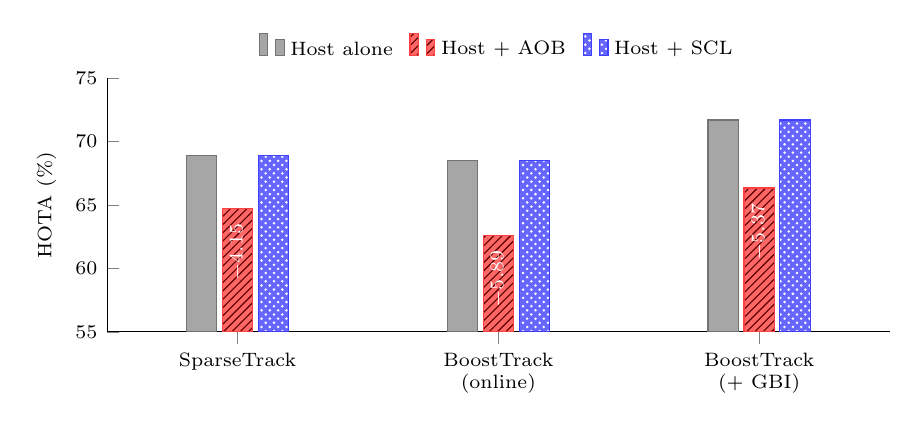
\begin{tikzpicture}
\begin{axis}[
  ybar,
  /pgf/bar width=11pt,
  width=0.95\columnwidth,
  height=4.8cm,
  ymin=55, ymax=75,
  xmin=0.5, xmax=3.5,
  xtick={1,2,3},
  xticklabels={SparseTrack, {BoostTrack\\(online)}, {BoostTrack\\(+ GBI)}},
  xticklabel style={align=center},
  ylabel={HOTA (\%)},
  axis x line*=bottom,
  axis y line*=left,
  tick label style={font=\scriptsize},
  label style={font=\scriptsize},
  legend style={at={(0.5,1.03)}, anchor=south, legend columns=3,
    font=\scriptsize, draw=none, /tikz/every even column/.append style={column sep=4pt}},
  legend cell align=left,
]
\addplot[fill=black!35, draw=black!55] coordinates {(1,68.88) (2,68.49) (3,71.72)};
\addplot[fill=red!60, draw=red!75, postaction={pattern=north east lines, pattern color=red!35!black}] coordinates {(1,64.72) (2,62.61) (3,66.35)};
\addplot[fill=blue!60, draw=blue!75, postaction={pattern=crosshatch dots, pattern color=white}] coordinates {(1,68.93) (2,68.49) (3,71.72)};
\legend{Host alone, Host + \aob{}, Host + \scl{}}
\node[rotate=90, anchor=east, font=\scriptsize, text=white] at (axis cs:1,64.3) {$-4.15$};
\node[rotate=90, anchor=east, font=\scriptsize, text=white] at (axis cs:2,62.2) {$-5.89$};
\node[rotate=90, anchor=east, font=\scriptsize, text=white] at (axis cs:3,65.9) {$-5.37$};
\end{axis}
\end{tikzpicture}

\caption{HOTA on MOT17 val-half of strong published trackers (SparseTrack and
BoostTrack in two settings) alone, with \aob{}, and with \scl{}. The labels
give the change caused by \aob{}}
\label{fig:prior}
\end{figure}

\subsection{Design steps}\label{sec:steps}
Each step from \aob{} to \scl{} was made to remove one cause found before it,
and it was compared with the step before it on development data
(Table~\ref{tab:ablation}). The steps, in the order in which they were made,
were the following.
\begin{itemize}
\item \emph{Starting point.} Running \aob{} inside the new framework showed
      the same problem: it reduced ByteTrack at floor 0.1 from 67.70 to 56.41
      HOTA and OC-SORT from 66.44 to 45.72.
\item \emph{Mode gate.} The two causes found in Sect.~\ref{sec:prior} were
      thresholds stricter than the trackers' own and the removal of hidden
      people as duplicates. The mode gate adds the mode check, the clean mode
      that keeps the tracker's settings, and the crowd-safe duplicate rule. It
      restored SparseTrack from 64.72 to 68.93 and BoostTrack from 62.61
      to 68.37.
\item \emph{Whole-stream mode.} The mode still changed in the middle of some
      streams. Choosing it from the whole stream removed these changes and
      raised ByteTrack from 67.561 to 67.702 and OC-SORT from 65.697 to
      66.071.
\item \emph{Continuation rescue.} Single-stage trackers still lost tracks
      whose objects got low scores for a few frames. The rescue added 0.2 to
      0.4 points for OC-SORT.
\item \emph{Background check.} Streams with few low-score candidates need a
      separate rule (Sect.~\ref{sec:calib}). The background check
      completed \scl{}: it returned ByteTrack and BoostTrack to output
      identical to the host and raised OC-SORT to 67.04 and 66.91 at the two
      floors.
\end{itemize}
Four other variants were also tested at these steps and were not kept
(Table~\ref{tab:ablation}).

\emph{What this stage showed.} After these steps, the layer kept the strong
two-stage trackers at their own accuracy and improved the single-stage
OC-SORT. This is the behavior that the frozen configuration was then tested
for on new trackers, detectors, and data (Sect.~\ref{sec:results}).

\begin{table*}[t]
\caption{Design steps from \aob{} to \scl{} on development
data (HOTA, \%), and versions that were tested and rejected. The floor of
ByteTrack and OC-SORT is given in parentheses.}
\label{tab:ablation}
\centering\footnotesize
\setlength{\tabcolsep}{4pt}
\begin{tabular}{@{}>{\raggedright\arraybackslash}p{25mm}>{\raggedright\arraybackslash}p{36mm}>{\raggedright\arraybackslash}p{62mm}@{}}
\toprule
Step & Change & Effect\\
\midrule
\aob{} emulated & always-noisy bands, overlap deduplication, rank remap & ByteTrack (0.1) 56.41 vs host 67.70; OC-SORT (0.1) 45.72 vs 66.44\\
+ mode gate & mode statistic, host-anchored clean mode, crowd-safe duplicates & SparseTrack 64.72 to 68.93 (host 68.88); BoostTrack 62.61 to 68.37 (host 68.49)\\
+ whole-stream mode & mode from all past frames & ByteTrack (0.1) 67.561 to 67.702; OC-SORT (0.1) 65.697 to 66.071\\
+ continuation rescue & foreground track-consistent rescue & OC-SORT (0.01) 66.405 to 66.619; OC-SORT (0.1) 66.071 to 66.469\\
+ background check = \scl{} & no background mode gives no evidence against the host & ByteTrack/BoostTrack (0.1) identical to host; OC-SORT 67.041 (0.01), 66.907 (0.1)\\
\midrule
\multicolumn{2}{@{}l}{\textit{Rejected version}} & \textit{Evidence}\\
\multicolumn{2}{@{}l}{no candidates at frame 1} & $-0.3$ to $-0.5$ HOTA on every MOT17 host\\
\multicolumn{2}{@{}l}{rescue below a two-stage host's low stage} & FP $+700$ to $+1000$, $-0.4$ to $-0.5$ HOTA\\
\multicolumn{2}{@{}l}{rank-remapped scores in clean frames} & ByteTrack $-0.2$ / $-1.6$ HOTA\\
\multicolumn{2}{@{}l}{host-clipped noisy primary band} & KITTI YOLOv8n ByteTrack $+1.4$ HOTA but uncontrolled false tracks on a noisy aerial stream (26.9 vs 14.9 boxes/frame)\\
\bottomrule
\end{tabular}
\end{table*}


\subsection{Freezing and testing}\label{sec:freeze}
The final configuration was frozen before any external test. It was saved as
a fixed, named version of the code (a version-control tag) and protected by a
lock file that stores a fingerprint (cryptographic hash) of the layer, its
configuration, and the evaluation scripts, so that any later change would be
detected. Every later run checked the lock before running. Sixty-one automated tests check
that the layer uses no future data, that its state resets between sequences,
that clean streams pass through unchanged, that the output does not depend on
detector, tracker, or sequence names, that stretching or shifting all logits
leaves the groups unchanged where designed, and that the lock is intact.

\section{Experimental Setup}\label{sec:setup}

The experiments test three expectations from the design. A tracker that
already fits its detector should keep its accuracy. A tracker that does not
fit, because it has no continuation step or because the detector or its
score scale changed, should gain. Both should hold on trackers and data that
were not seen during design.

\label{sec:hosts}Seven published trackers serve as hosts: ByteTrack
\cite{zhang2022bytetrack}, BoT-SORT \cite{aharon2022botsort}, OC-SORT
\cite{cao2023ocsort}, SparseTrack \cite{liu2025sparsetrack}, BoostTrack
\cite{stanojevic2024boosttrack}, PD-SORT \cite{wang2025pdsort}, and
Hybrid-SORT \cite{yang2024hybridsort}. Each host uses the authors' code and
published configuration, and its contract is given in
Table~\ref{tab:contracts}.

In every comparison the baseline is the host alone, called Host in the
tables: the published tracker without \scl{}, run by us with its published
configuration and the same detections. The
second run adds the frozen \scl{} and changes nothing else. Both runs use the
same environment. Where the authors report their own numbers, these are
listed next to our reproduction of the host.

\section{Results and Analysis}\label{sec:results}

Figure~\ref{fig:forest} shows the HOTA difference between each host with
\scl{} and the host alone for every tested cell. The next subsections give
the baseline comparison for each part of the evaluation, in the order of the
three expectations of Sect.~\ref{sec:setup}: well-matched trackers, trackers
that do not fit their detector, and systems not seen during design.

\begin{figure}[t]
\centering
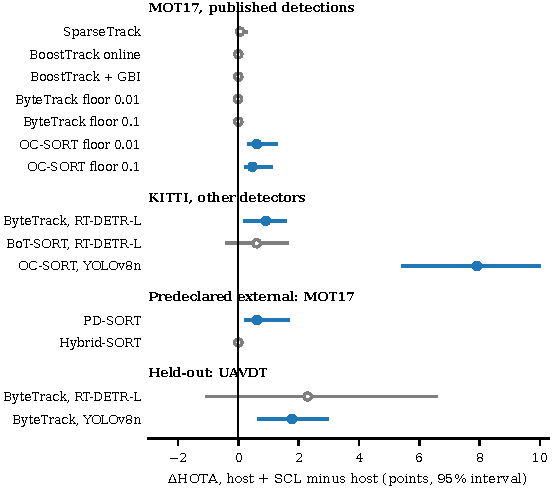
\includegraphics[width=\columnwidth]{fig3_forest_col.pdf}
\caption{Difference in HOTA (host with \scl{} minus host alone) with
95\% paired-bootstrap interval for every tested cell. Filled blue circles:
interval above zero; open gray circles: interval contains zero, or identical
output}
\label{fig:forest}
\end{figure}

\subsection{Results across trackers}\label{sec:tracker}
Table~\ref{tab:mot17} compares the development trackers with their hosts on
MOT17. The two-stage trackers with well-matched detections stayed at the
accuracy of their hosts. BoostTrack, online and with GBI, and
ByteTrack at floor 0.1 gave exactly the same output as without the layer, and ByteTrack at floor 0.01 and
SparseTrack stayed within 0.06 HOTA points of their hosts ($-0.014$ and
$+0.055$). This is the
self-limiting behavior of the clean mode (Sect.~\ref{sec:regimes}), which
the earlier design did not have (Table~\ref{tab:prior}).

The single-stage OC-SORT improved at both emission floors. Its HOTA rose by
0.61 points ($[+0.36,+1.24]$) at floor 0.01 and by 0.46 points
($[+0.27,+1.09]$) at floor 0.1, and its MOTA by 1.27 and 1.26 points. Its identity switches also fell, by 8
at floor 0.01 ($[-15,-2]$) and by 14 at floor 0.1. HOTA
was higher on 7 of 7 sequences in both settings (Fig.~\ref{fig:perseq}). The
gain comes from the continuation rescue. OC-SORT drops every detection
below its single threshold, and the layer passes it the foreground candidates
that continue a track that would otherwise stay unmatched.

\begin{table}[t]
\caption{Baseline comparison of the development trackers on MOT17 val-half
(published YOLOX-X detections). Paper: number reported by the tracker's
authors. Host: the tracker alone, without \scl{} (our run of the published tracker). $\Delta$: host with
\scl{} minus host, with 95\% paired-bootstrap interval (10,000
resamples, seed 42); bold intervals exclude zero. The floor is the lowest
detector score emitted. IDS: identity switches, a count (lower is better);
--: not reported by the authors.}
\label{tab:mot17}
\centering\footnotesize
\setlength{\tabcolsep}{4pt}
\begin{tabular}{@{}lrrl@{}}
\toprule
Metric & Paper & Host & $\Delta$ [95\% CI]\\
\midrule
\multicolumn{4}{@{}l}{\textit{SparseTrack} \cite{liu2025sparsetrack}}\\
\quad HOTA & 69.2 & 68.88 & $+0.06$ [$-0.01$, $+0.25$]\\
\quad MOTA & 76.8 & 77.85 & $+0.08$ [$-0.03$, $+0.30$]\\
\quad IDF1 & 81.4 & 81.97 & $+0.16$ [$-0.02$, $+0.70$]\\
\quad IDS & -- & 124 & $+7$ [$0$, $+19$]\\
\multicolumn{4}{@{}l}{\textit{BoostTrack, online} \cite{stanojevic2024boosttrack}}\\
\quad HOTA & 68.37 & 68.49 & 0 (identical)\\
\quad MOTA & 75.56 & 75.50 & 0 (identical)\\
\quad IDF1 & 81.35 & 81.41 & 0 (identical)\\
\quad IDS & 118 & 113 & 0 (identical)\\
\multicolumn{4}{@{}l}{\textit{BoostTrack, + GBI} \cite{stanojevic2024boosttrack}}\\
\quad HOTA & 71.33 & 71.72 & 0 (identical)\\
\quad MOTA & 80.55 & 81.03 & 0 (identical)\\
\quad IDF1 & 83.84 & 84.16 & 0 (identical)\\
\quad IDS & 106 & 97 & 0 (identical)\\
\multicolumn{4}{@{}l}{\textit{ByteTrack, floor 0.01} \cite{zhang2022bytetrack}}\\
\quad HOTA & -- & 67.70 & $-0.014$ [$-0.058$, $+0.009$]\\
\quad MOTA & 76.6 & 77.60 & $+0.06$ [$-0.15$, $+0.34$]\\
\quad IDF1 & 79.3 & 79.47 & $-0.031$ [$-0.135$, $+0.035$]\\
\quad IDS & -- & 214 & $+4$ [$-2$, $+13$]\\
\multicolumn{4}{@{}l}{\textit{ByteTrack, floor 0.1} \cite{zhang2022bytetrack}}\\
\quad HOTA & -- & 67.70 & 0 (identical)\\
\quad MOTA & 76.6 & 77.60 & 0 (identical)\\
\quad IDF1 & 79.3 & 79.47 & 0 (identical)\\
\quad IDS & -- & 214 & 0 (identical)\\
\multicolumn{4}{@{}l}{\textit{OC-SORT, floor 0.01} \cite{cao2023ocsort}}\\
\quad HOTA & 66.5 & 66.43 & {\boldmath $+0.61$ [$+0.36$, $+1.24$]}\\
\quad MOTA & 74.9 & 74.67 & {\boldmath $+1.27$ [$+0.17$, $+3.01$]}\\
\quad IDF1 & 77.7 & 78.05 & $+0.66$ [$-0.25$, $+1.60$]\\
\quad IDS & -- & 211 & {\boldmath $-8$ [$-15$, $-2$]}\\
\multicolumn{4}{@{}l}{\textit{OC-SORT, floor 0.1} \cite{cao2023ocsort}}\\
\quad HOTA & 66.5 & 66.44 & {\boldmath $+0.46$ [$+0.27$, $+1.09$]}\\
\quad MOTA & 74.9 & 74.67 & {\boldmath $+1.26$ [$+0.37$, $+3.34$]}\\
\quad IDF1 & 77.7 & 78.05 & {\boldmath $+0.287$ [$+0.003$, $+0.838$]}\\
\quad IDS & -- & 213 & $-14$ [$-38$, $+6$]\\
\bottomrule
\end{tabular}
\end{table}


\begin{figure}[t]
\centering
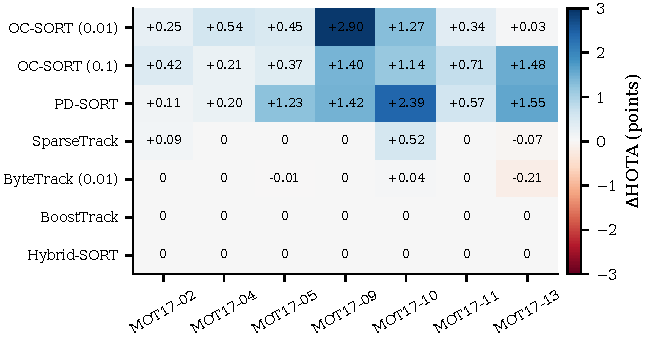
\includegraphics[width=\columnwidth]{fig4_per_sequence.pdf}
\caption{Per-sequence HOTA differences (host with \scl{} minus host
alone) on MOT17 val-half for the development and predeclared trackers}
\label{fig:perseq}
\end{figure}

\subsection{Results with other detectors}\label{sec:detector}
Table~\ref{tab:kitti} reports the KITTI results with the two other detectors. With
the noisy RT-DETR-L detector, the two-stage trackers gained in MOTA and IDF1.
ByteTrack gained 5.98 MOTA points ($[+1.16,+9.94]$), 3.87 IDF1 points, and
0.91 HOTA points ($[+0.22,+1.55]$). BoT-SORT gained 7.86 MOTA points
($[+2.21,+13.44]$) and 3.10 IDF1 points. Both also had fewer identity switches: 297
fewer for ByteTrack and 226 fewer for BoT-SORT. With YOLOv8n, the single-stage
OC-SORT gained 7.91 HOTA points ($[+5.47,+9.98]$), 9.40 MOTA points, and 9.60
IDF1 points. It had 79 more identity switches, because it now followed many
more objects: its missed objects (FN) fell from 21,886 to 16,576, and its IDF1,
which measures how well identities are kept, rose.

\begin{table}[t]
\caption{Baseline comparison under a detector change on KITTI tracking
training (official HOTA, car and pedestrian averaged). Host: the tracker
alone, without \scl{}, with the same detections. $\Delta$: host with \scl{}
minus host, with 95\% paired-bootstrap interval; bold intervals exclude zero.
IDS: identity switches, a count (lower is better).}
\label{tab:kitti}
\centering\footnotesize
\setlength{\tabcolsep}{4pt}
\begin{tabular}{@{}lrl@{}}
\toprule
Metric & Host & $\Delta$ [95\% CI]\\
\midrule
\multicolumn{3}{@{}l}{\textit{ByteTrack} \cite{zhang2022bytetrack}\textit{, RT-DETR-L}}\\
\quad HOTA & 50.73 & {\boldmath $+0.91$ [$+0.22$, $+1.55$]}\\
\quad MOTA & 47.27 & {\boldmath $+5.98$ [$+1.16$, $+9.94$]}\\
\quad IDF1 & 64.98 & {\boldmath $+3.87$ [$+1.67$, $+5.06$]}\\
\quad IDS & 686 & {\boldmath $-297$ [$-530$, $-122$]}\\
\multicolumn{3}{@{}l}{\textit{BoT-SORT} \cite{aharon2022botsort}\textit{, RT-DETR-L} (20 sequences)}\\
\quad HOTA & 53.91 & $+0.61$ [$-0.39$, $+1.61$]\\
\quad MOTA & 48.25 & {\boldmath $+7.86$ [$+2.21$, $+13.44$]}\\
\quad IDF1 & 67.74 & {\boldmath $+3.10$ [$+1.00$, $+4.57$]}\\
\quad IDS & 476 & {\boldmath $-226$ [$-369$, $-120$]}\\
\multicolumn{3}{@{}l}{\textit{OC-SORT} \cite{cao2023ocsort}\textit{, YOLOv8n}}\\
\quad HOTA & 36.27 & {\boldmath $+7.91$ [$+5.47$, $+9.98$]}\\
\quad MOTA & 33.99 & {\boldmath $+9.40$ [$+1.10$, $+12.30$]}\\
\quad IDF1 & 50.46 & {\boldmath $+9.60$ [$+5.61$, $+12.16$]}\\
\quad IDS & 91 & {\boldmath $+79$ [$+43$, $+125$]}\\
\bottomrule
\end{tabular}
\end{table}


\subsection{Results under shifted detector scores}\label{sec:shift}
Table~\ref{tab:shift} and Fig.~\ref{fig:shift} show the trackers under the
four score transforms. Halving the scores reduced ByteTrack (official setting)
and OC-SORT to 0 HOTA, because no detection reached their thresholds. With the
layer they reached 66.17 and 66.72. Cubing reduced them to 60.92 and 58.34,
and the layer restored them to 65.81 and 66.60. BoostTrack rose from 61.33 to
64.84 under cubing. With temperature $T=2$, the layer raised ByteTrack and
OC-SORT by 1.11 and 1.24 points. The library setting of ByteTrack, whose low
thresholds already accept the changed scores, stayed within 0.14 points in all
four transforms. Over the 14 conditions, the layer raised HOTA significantly
in 7 and lowered it significantly in none. When a transform made a host lose
most of its detections, the host also had few identity switches, because it
followed few objects; under halved scores it followed none, so it had 0.

\begin{table*}[t]
\caption{Baseline comparison under shifted detector scores on MOT17 val-half. The detector
scores are transformed before the tracker, whose published thresholds stay fixed; $T$ is a logit
temperature, $\sigma(z/T)$. Host: the tracker alone, without \scl{}. $\Delta$: with \scl{} minus host,
with 95\% paired-bootstrap interval (10,000 resamples, seed 42); bold intervals exclude zero.
IDS: identity switches, a count (lower is better). A host that loses most detections also has
few identity switches, because it follows few objects (for example 0 HOTA and 0 IDS under halved
scores). Emission floor 0.01 (BoostTrack 0.1).}
\label{tab:shift}
\centering\footnotesize
\setlength{\tabcolsep}{5pt}
\begin{tabular}{@{}lrrlrr@{}}
\toprule
 & \multicolumn{3}{c}{HOTA (\%)} & \multicolumn{2}{c}{IDS}\\
\cmidrule(lr){2-4}\cmidrule(l){5-6}
Transform & Host & + \scl{} & $\Delta$ [95\% CI] & Host & + \scl{}\\
\midrule
\multicolumn{6}{@{}l}{\textit{ByteTrack, official setting} \cite{zhang2022bytetrack}}\\
\quad $s^3$ & 60.92 & 65.81 & {\boldmath $+4.89$ [$+2.60$, $+13.69$]} & 48 & 250\\
\quad $0.5\,s$ & 0.00 & 66.17 & {\boldmath $+66.17$ [$+49.32$, $+75.40$]} & 0 & 298\\
\quad $T=2$ & 65.84 & 66.95 & {\boldmath $+1.11$ [$+0.35$, $+3.87$]} & 97 & 172\\
\quad $T=0.5$ & 67.30 & 67.29 & $-0.009$ [$-0.051$, $+0.005$] & 229 & 229\\
\multicolumn{6}{@{}l}{\textit{ByteTrack, library setting} \cite{zhang2022bytetrack}}\\
\quad $s^3$ & 66.31 & 66.31 & $-0.006$ [$-0.384$, $+0.383$] & 240 & 265\\
\quad $0.5\,s$ & 66.61 & 66.48 & $-0.14$ [$-0.66$, $+0.14$] & 297 & 302\\
\quad $T=2$ & 63.97 & 63.97 & 0 (identical) & 470 & 470\\
\quad $T=0.5$ & 66.53 & 66.52 & $-0.006$ [$-0.029$, $+0.001$] & 387 & 388\\
\multicolumn{6}{@{}l}{\textit{OC-SORT} \cite{cao2023ocsort}}\\
\quad $s^3$ & 58.34 & 66.60 & {\boldmath $+8.26$ [$+5.86$, $+16.81$]} & 98 & 235\\
\quad $0.5\,s$ & 0.00 & 66.72 & {\boldmath $+66.72$ [$+50.32$, $+75.56$]} & 0 & 260\\
\quad $T=2$ & 65.99 & 67.22 & {\boldmath $+1.24$ [$+0.52$, $+3.42$]} & 171 & 154\\
\quad $T=0.5$ & 66.61 & 67.06 & $+0.45$ [$-0.01$, $+0.97$] & 223 & 231\\
\multicolumn{6}{@{}l}{\textit{BoostTrack, online} \cite{stanojevic2024boosttrack}}\\
\quad $s^3$ & 61.33 & 64.84 & {\boldmath $+3.51$ [$+0.85$, $+13.28$]} & 76 & 166\\
\quad $T=2$ & 67.59 & 67.59 & 0 (identical) & 119 & 119\\
\bottomrule
\end{tabular}
\end{table*}


\begin{figure*}[t]
\centering
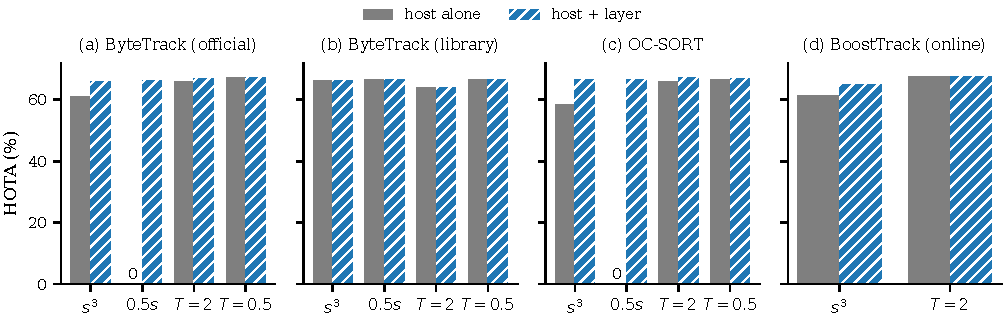
\includegraphics[width=0.9\textwidth]{fig5_calibration_shift.pdf}
\caption{Shifted detector scores on MOT17 val-half: HOTA of each published
tracker with its published thresholds, alone and with \scl{}, after
four monotone transforms of the detector scores ($s^3$, $0.5\,s$, and
temperatures $T=2$ and $T=0.5$). (a) ByteTrack, official setting;
(b) ByteTrack, library setting; (c) OC-SORT; (d) BoostTrack, online. Hatched bars:
host with \scl{}}
\label{fig:shift}
\end{figure*}

\subsection{Comparison with adaptive-threshold methods}\label{sec:baselines}
A simpler way to follow the detector scores is to set the tracker's
thresholds from them directly. Two such baselines were built on the same
input and with the same window of the last 10 frames. They set the tracker's
matching and birth thresholds in every frame to the first or the second Otsu
split of the recent logits, $t_1$ or $t_2$, and pass the scores unchanged,
without the mode decision, the new scores, or the rescue.
Table~\ref{tab:baselines} compares them with \scl{} on KITTI, for OC-SORT
with YOLOv8n and for both trackers under halved scores. \scl{} reached the
highest HOTA in all three cells, 2.2 to 8.6 points above the two baselines,
and its paired-bootstrap intervals against the $t_2$ baseline lie
above zero in every cell. Adaptive thresholds alone therefore do not explain
the gains; the other parts of the layer add to them. With OC-SORT and
YOLOv8n, \scl{} also had fewer identity switches than both baselines (170
against 1,545 and 250). Under halved scores, ByteTrack with \scl{} had more
(501 against 273 and 275), while it missed far fewer objects (FN 7,750 against
12,357 with the $t_2$ baseline).

\emph{Comparison with a published method.} ACT \cite{act2026adaptive} sets the
high and low thresholds of a two-stage tracker in every frame from the first
quartile and the number of the current scores, using fixed score levels. It
was run with its published parameters on the same detections as \scl{}, in
three settings (Table~\ref{tab:act}): KITTI with halved scores, for ByteTrack
and, with its high threshold as the single threshold, for OC-SORT; its own
setting, MOT17 val-half with ByteTrack's official setting and the YOLOX-X
detections; and the held-out UAVDT test split with ByteTrack. \scl{} reached
higher HOTA than ACT in every row of Table~\ref{tab:act}. The difference was
significant under halved scores ($+2.01$ and $+10.06$ points) and with
YOLOv8n on UAVDT ($+1.82$ points, with $+4.00$ points of IDF1). In the setting
of ACT itself, the two were close ($+0.22$ and $+0.23$ points). With RT-DETR-L
on UAVDT, \scl{} reached a MOTA of 27.99 against 5.34 for ACT (difference
$+22.65$, [$+9.03$, $+47.21$]): the host produced many false positives, and
the fixed levels of ACT removed few of them (178,219 false positives, against
78,975 with \scl{}). \scl{} also had fewer identity switches than ACT on MOT17 and UAVDT,
significantly with RT-DETR-L on UAVDT (418 fewer). Under halved scores on
KITTI it had more (240 and 214 more), because it followed many more objects:
it missed 7,750 objects against 12,326 for ACT with ByteTrack, and 13,547
against 21,887 with OC-SORT. The levels of ACT are fixed scores, so they do
not move when the scores shift, while the splits of \scl{} are computed on
the scores themselves.

\emph{Contribution of each part.} Removing one part of the frozen \scl{} at
a time shows where the gains come from, on the KITTI cells. Without the
continuation rescue, the HOTA of OC-SORT fell by 3.34 points with YOLOv8n and
by 1.16 points under halved scores. Using the clean mode in every frame,
that is, without the mode decision, lowered HOTA by 0.90 points
for ByteTrack with RT-DETR-L and by 2.40 and 2.44 points for the two trackers
under halved scores. Without the new scores of the noisy mode, HOTA fell by
1.67 and 0.61 points under halved scores.

\begin{table*}[t]
\caption{HOTA and identity switches of \scl{} and of two simple adaptive-threshold baselines on
KITTI tracking training (official HOTA, car and pedestrian averaged). Host: the tracker alone,
without any layer. Adaptive $t_1$, $t_2$: the
tracker's matching and birth thresholds are set in every frame to the first or second Otsu split of
the logits of the last 10 frames, and the scores are passed unchanged. $\Delta$: \scl{} minus the
adaptive $t_2$ baseline, with 95\% paired-bootstrap interval; bold intervals exclude zero. IDS:
identity switches, a count (lower is better); a host with 0 HOTA follows no object, so it also has
0 IDS.}
\label{tab:baselines}
\centering\footnotesize
\setlength{\tabcolsep}{4pt}
\begin{tabular}{@{}lrrrrlrrrr@{}}
\toprule
 & \multicolumn{5}{c}{HOTA (\%)} & \multicolumn{4}{c}{IDS}\\
\cmidrule(lr){2-6}\cmidrule(l){7-10}
Cell & Host & Adapt.\ $t_1$ & Adapt.\ $t_2$ & \scl{} & $\Delta$ [95\% CI] & Host & Adapt.\ $t_1$ & Adapt.\ $t_2$ & \scl{}\\
\midrule
\twol{OC-SORT, YOLOv8n}{} & 36.27 & 39.97 & 41.09 & 44.17 & {\boldmath $+3.09$ [$+2.00$, $+4.03$]} & 91 & 1545 & 250 & 170\\
\addlinespace[4pt]
\twol{ByteTrack, RT-DETR-L,}{halved scores} & 49.50 & 49.58 & 49.50 & 51.78 & {\boldmath $+2.29$ [$+0.28$, $+4.96$]} & 279 & 273 & 275 & 501\\
\addlinespace[4pt]
\twol{OC-SORT, YOLOv8n,}{halved scores} & 0.00 & 37.68 & 43.56 & 46.30 & {\boldmath $+2.74$ [$+1.32$, $+3.34$]} & 0 & 1975 & 492 & 308\\
\bottomrule
\end{tabular}
\end{table*}

\begin{table*}[t]
\caption{HOTA of ACT \cite{act2026adaptive} and of \scl{} on the same detections, and the
differences \scl{} minus ACT in HOTA, IDF1, and identity switches (IDS, a count; lower is better),
with 95\% paired-bootstrap interval below each value; bold intervals exclude zero. ACT: published parameters, no
tuning. KITTI: official HOTA, car and pedestrian averaged; MOT17: val-half, ACT's own setting;
UAVDT: the protocol of Table~\ref{tab:visdrone}.}
\label{tab:act}
\centering\footnotesize
\setlength{\tabcolsep}{3pt}
\begin{tabular}{@{}lllrrccc@{}}
\toprule
Data & Detector & Tracker & ACT & \scl{} & $\Delta$HOTA & $\Delta$IDF1 & $\Delta$IDS\\
\midrule
KITTI, halved scores & RT-DETR-L & ByteTrack & 49.77 & 51.78 & \cib{+2.01}{+0.01}{+4.76} & \ci{+1.70}{-1.13}{+6.80} & \cib{+240}{+94}{+401}\\
KITTI, halved scores & YOLOv8n & OC-SORT & 36.24 & 46.30 & \cib{+10.06}{+6.88}{+12.01} & \cib{+12.03}{+6.85}{+14.69} & \cib{+214}{+141}{+295}\\
\addlinespace[4pt]
MOT17, floor 0.01 & YOLOX-X & ByteTrack (official) & 67.46 & 67.68 & \ci{+0.22}{-0.43}{+0.88} & \ci{+0.57}{-0.68}{+2.12} & \ci{-18}{-62}{+12}\\
MOT17, floor 0.1 & YOLOX-X & ByteTrack (official) & 67.46 & 67.70 & \ci{+0.23}{-0.40}{+0.90} & \ci{+0.60}{-0.55}{+2.10} & \ci{-22}{-61}{+4}\\
\addlinespace[4pt]
UAVDT test & YOLOv8n & ByteTrack & 29.01 & 30.83 & \cib{+1.82}{+0.65}{+3.00} & \cib{+4.00}{+1.85}{+6.22} & \ci{-185}{-480}{+13}\\
UAVDT test & RT-DETR-L & ByteTrack & 40.14 & 42.37 & \ci{+2.23}{-0.97}{+6.32} & \ci{+5.35}{-0.03}{+12.47} & \cib{-418}{-718}{-123}\\
\bottomrule
\end{tabular}
\end{table*}


\subsection{Results on external trackers}\label{sec:external}
Table~\ref{tab:external} gives the two predeclared external systems. PD-SORT
\cite{wang2025pdsort} was reproduced exactly as in the authors' released
output. With \scl{}, its HOTA rose by 0.61 points ($[+0.27,+1.65]$), its
MOTA by 1.13 points ($[+0.27,+3.03]$), and its IDF1 by 0.82 points
($[+0.43,+1.94]$), with higher HOTA on 7 of 7 sequences
(Fig.~\ref{fig:perseq}). FN fell by 1,291, FP rose by 681, and the identity switches stayed almost the
same (131 against 129). PD-SORT is a single-stage tracker, and its gain comes from the same
step as for OC-SORT; unlike OC-SORT, it was not seen during design.
Hybrid-SORT \cite{yang2024hybridsort}, a two-stage tracker, gave identical
output, as predicted before the run.

\begin{table}[t]
\caption{Baseline comparison on the predeclared external systems (MOT17
val-half, authors' released detections), each evaluated once with the frozen
\scl{}. Paper: number reported by the authors (for PD-SORT, their released
output). Host: the tracker alone, without \scl{} (our run of the published tracker). Reproduction class
against the authors' number (EXACT: $|\Delta\mathrm{HOTA}|\le0.2$; CLOSE:
$\le1.0$ with a documented, untuned cause). $\Delta$: host with \scl{} minus
host, with 95\% paired-bootstrap interval; bold intervals exclude zero. IDS:
identity switches, a count (lower is better); --: not reported.}
\label{tab:external}
\centering\footnotesize
\setlength{\tabcolsep}{4pt}
\begin{tabular}{@{}lrrl@{}}
\toprule
Metric & Paper & Host & $\Delta$ [95\% CI]\\
\midrule
\multicolumn{4}{@{}l}{\textit{PD-SORT} \cite{wang2025pdsort}\textit{, EXACT}}\\
\quad HOTA & 68.01 & 68.01 & {\boldmath $+0.61$ [$+0.27$, $+1.65$]}\\
\quad MOTA & 75.19 & 75.19 & {\boldmath $+1.13$ [$+0.27$, $+3.03$]}\\
\quad IDF1 & 81.03 & 81.03 & {\boldmath $+0.82$ [$+0.43$, $+1.94$]}\\
\quad IDS & -- & 129 & $+2$ [$-9$, $+13$]\\
\multicolumn{4}{@{}l}{\textit{Hybrid-SORT} \cite{yang2024hybridsort}\textit{, CLOSE}}\\
\quad HOTA & 67.1 & 66.70 & 0 (identical)\\
\quad MOTA & 75.8 & 75.52 & 0 (identical)\\
\quad IDF1 & 78.0 & 77.56 & 0 (identical)\\
\quad IDS & -- & 259 & 0 (identical)\\
\bottomrule
\end{tabular}
\end{table}


\subsection{Results on held-out aerial data}\label{sec:visdrone}
Table~\ref{tab:visdrone} gives the held-out UAVDT test split. \scl{} raised the HOTA of the YOLOv8n stream by 1.77 points
($[+0.70,+2.94]$) and its IDF1 by 3.97 points ($[+1.88,+6.17]$), and
identity switches fell by 45\% (from 719 to 393). With RT-DETR-L, the host produced many false
positives (MOTA 3.29); with \scl{}, its MOTA rose by 24.70 points
($[+10.06,+51.08]$) and its IDF1 by 5.74 points ($[+0.13,+13.11]$): false
positives fell by 58\% and identity switches by 56\% (from 1,041 to 455). HOTA did not fall with either
detector.

\begin{table}[t]
\caption{Baseline comparison on the held-out UAVDT test split (20 aerial
sequences, not used during design), evaluated once with the frozen \scl{}. Host: ByteTrack alone, without \scl{}, with its published setting. $\Delta$: host
with \scl{} minus host, with 95\% paired-bootstrap interval; bold intervals
exclude zero. IDS: identity switches, a count (lower is better).}
\label{tab:visdrone}
\centering\footnotesize
\setlength{\tabcolsep}{4pt}
\begin{tabular}{@{}lrl@{}}
\toprule
Metric & Host & $\Delta$ [95\% CI]\\
\midrule
\multicolumn{3}{@{}l}{\textit{ByteTrack, RT-DETR-L} \cite{zhang2022bytetrack,zhao2024rtdetr}}\\
\quad HOTA & 40.07 & $+2.30$ [$-1.05$, $+6.55$]\\
\quad MOTA & 3.29 & {\boldmath $+24.70$ [$+10.06$, $+51.08$]}\\
\quad IDF1 & 48.59 & {\boldmath $+5.74$ [$+0.13$, $+13.11$]}\\
\quad IDS & 1041 & {\boldmath $-586$ [$-951$, $-248$]}\\
\multicolumn{3}{@{}l}{\textit{ByteTrack, YOLOv8n} \cite{zhang2022bytetrack,jocher2023yolov8}}\\
\quad HOTA & 29.05 & {\boldmath $+1.77$ [$+0.70$, $+2.94$]}\\
\quad MOTA & 16.27 & $+1.02$ [$-1.06$, $+2.86$]\\
\quad IDF1 & 34.52 & {\boldmath $+3.97$ [$+1.88$, $+6.17$]}\\
\quad IDS & 719 & {\boldmath $-326$ [$-691$, $-73$]}\\
\bottomrule
\end{tabular}
\end{table}


\subsection{Running time}\label{sec:latency}
\label{sec:latency-setup}Running time was measured after the freeze on one cloud machine with a 4-vCPU
Intel Xeon processor at 2.10 GHz, 15 GB of memory, and no graphics processing unit (GPU). A live YOLOv8n
detector (32-bit floats, 736 pixels, batch 1) feeds ByteTrack on three KITTI
tracking sequences (0001, 0009, and 0019). Both runs use the same frames
one after the other, and the first ten frames of each sequence are excluded,
which leaves 2,279 timed frames per run. The time of the layer includes the
motion cue, the per-frame step, and saving the tracker output.

Table~\ref{tab:runtime} and Fig.~\ref{fig:runtime} compare the time per frame
of the host pipeline with and without \scl{}. \scl{} took 2.95 ms per
frame on average and 4.39 ms at the 95th percentile (95\% of the frames took
less time), including the
phase-correlation motion cue. The total time rose from 57.85 to 60.44 ms
per frame, by 4.5\%. The tracker became faster, from 2.04 to 1.43 ms per
frame, because it received fewer candidates. The detector takes most of each
frame, about 42 ms, so the layer adds only a small part of the total time.

\begin{table}[t]
\caption{Baseline comparison of the per-frame time on a 4-vCPU Intel Xeon
(2.10 GHz, no GPU) with a live YOLOv8n detector (736 pixels) and ByteTrack on
three KITTI sequences (2,279 timed frames per arm). Host alone: the same
pipeline without \scl{}. Mean / 95th percentile in milliseconds.}
\label{tab:runtime}
\centering\footnotesize
\setlength{\tabcolsep}{4pt}
\begin{tabular}{@{}lcc@{}}
\toprule
Stage & Host alone & Host + \scl{}\\
\midrule
Frame decode & 13.88 / 16.21 & 13.88 / 16.51\\
Detector (YOLOv8n, 736 px) & 41.91 / 58.41 & 42.17 / 59.43\\
\scl{} & -- & 2.95 / 4.39\\
Tracker (ByteTrack) & 2.04 / 3.57 & 1.43 / 2.64\\
End to end & 57.85 / 76.35 & 60.44 / 80.78\\
\bottomrule
\end{tabular}
\end{table}


\begin{figure}[t]
\centering
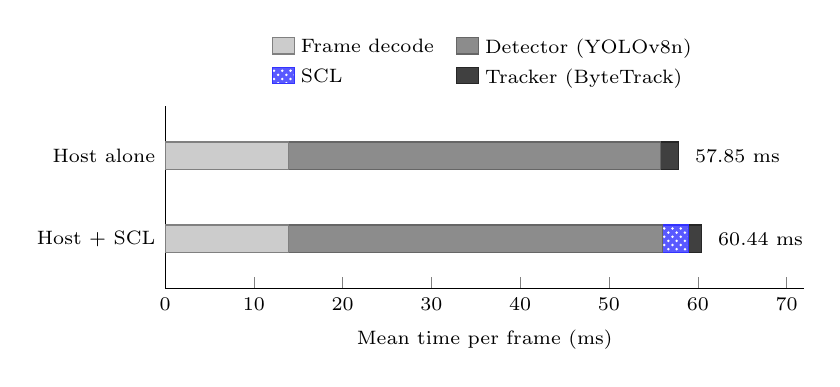
\begin{tikzpicture}
\begin{axis}[
  xbar stacked,
  /pgf/bar width=10pt,
  width=0.8\columnwidth,
  height=3.9cm,
  xmin=0, xmax=72,
  clip=false,
  ymin=-0.6, ymax=1.6,
  ytick={0,1},
  yticklabels={Host + \scl{}, Host alone},
  xlabel={Mean time per frame (ms)},
  axis x line*=bottom,
  axis y line*=left,
  tick label style={font=\scriptsize},
  label style={font=\scriptsize},
  legend style={at={(0.5,1.04)}, anchor=south, legend columns=2,
    font=\scriptsize, draw=none, /tikz/every even column/.append style={column sep=6pt}},
  legend cell align=left,
]
\addplot[fill=black!20, draw=black!50] coordinates {(13.88,1) (13.88,0)};
\addplot[fill=black!45, draw=black!60] coordinates {(41.91,1) (42.17,0)};
\addplot[fill=blue!65, draw=blue!80, postaction={pattern=crosshatch dots, pattern color=white}] coordinates {(0,1) (2.95,0)};
\addplot[fill=black!75, draw=black!85] coordinates {(2.04,1) (1.43,0)};
\legend{Frame decode, Detector (YOLOv8n), \scl{}, Tracker (ByteTrack)}
\node[anchor=west, font=\scriptsize] at (axis cs:58.6,1) {57.85 ms};
\node[anchor=west, font=\scriptsize] at (axis cs:61.2,0) {60.44 ms};
\end{axis}
\end{tikzpicture}

\caption{Mean per-frame time by stage for the host pipeline alone and with
\scl{} (4-vCPU Intel Xeon, no GPU). The labels give the measured
end-to-end time}
\label{fig:runtime}
\end{figure}

\subsection{Analysis}\label{sec:discussion}

\emph{When the layer acts.} The effect depends on two properties of the
pipeline, not on the dataset: whether the tracker has a continuation step,
and whether the detector's scores match the tracker's thresholds. On MOT17
with well-matched detections, the two-stage trackers BoostTrack, ByteTrack at
floor 0.1, and Hybrid-SORT produced output identical to their hosts, while
the single-stage OC-SORT and PD-SORT gained HOTA on every sequence. When the
stream fits the tracker, the layer stays out of the way, and when the
tracker lacks a step, the layer adds it.

\emph{Self-limiting by design.} In the clean mode the layer keeps the
tracker's thresholds and scores, so a tracker with a low-score step and
well-matched detections receives its normal input. This is the main
difference from the earlier design \aob{}, which lowered the HOTA of the same
strong trackers by 4.15 to 5.89 points (Table~\ref{tab:prior}). The layer
therefore does not need to know in advance whether a tracker needs help; it
reads the answer from the scores.

\emph{A continuation step for single-stage trackers.} Single-stage trackers
drop every detection below one threshold, so a track can be lost when its
object receives low scores for a few frames. The continuation rescue
considers only candidates that overlap a track of the previous frame that no
usable candidate covers, so it targets exactly these gaps. OC-SORT and the
external PD-SORT gained HOTA on 7 of 7 MOT17 sequences through this step.

\emph{Detector replacement.} When a detector is replaced or its score scale
shifts, the fixed thresholds of a tracker no longer match the scores. The
layer adjusts them from the scores without labels. Under halved scores it
restored two trackers from 0 to about 66 HOTA, with a different detector
it raised the MOTA of two two-stage trackers by 6.0 and 7.9 points, and on
held-out aerial data it raised the MOTA of ByteTrack with RT-DETR-L from 3.3
to 28.0. This is
the case the layer was built for: a detector that is swapped, retrained, or
quantized while the tracker stays the same.

\emph{Relation to detector-side control.} Our AC-MOT controller acts
before the detector and chooses its settings from the scene. \scl{}
acts after the detector and adapts the tracker's input to the scores that the
detector produces. The two layers work on different parts of the pipeline,
so they could be used together; combining them is left for future work.

\emph{Real-time use.} The layer needs no training, no GPU, and no access to
the inside of the detector, and it needs only four contract values from the
tracker's configuration. At run time it reads the candidate list, one small
grayscale image for the motion cue, and the tracks of the previous frame. On
a CPU it takes 2.95 ms per frame, adds 4.5\% to the total time, and makes the
tracker itself faster. \scl{} therefore adds very little delay and is
suitable for real-time use. New trackers are added through their published
contract values and an adapter, without changes to the rules.

\section{Conclusion}\label{sec:conclusion}

This paper presented \scl{}, a control layer that needs no training, adjusts
itself from a detector's scores, and adapts a frozen tracker through a
declared host contract. The layer splits the logits of recent frames with
nested Otsu thresholds and decides whether the stream is clean or noisy. On
clean streams it keeps the tracker's settings; on noisy streams it chooses
the candidates, assigns them new scores, and sets the thresholds. A
continuation rescue gives single-stage trackers the step they lack.

One frozen configuration, developed step by step from \aob{}, was tested on
seven published trackers, four detection sources, and three datasets. It
improved single-stage trackers and trackers whose detector or score scale had
changed, raised MOTA by 24.7 points on held-out aerial data, reached higher HOTA than
simple adaptive thresholds on the same scores and than the published ACT
method under halved scores and on held-out aerial data, kept well-matched two-stage
trackers at their own accuracy, showed no statistically significant HOTA loss
in any tested cell, and took 2.95 ms per frame on a CPU. These results support placing a self-calibrating
layer between the detector and the tracker in systems where the detector
changes while the tracker stays the same.


\backmatter

\section*{Statements and Declarations}

\bmhead{Funding}
The authors did not receive support from any organization for the submitted work.

\bmhead{Competing interests}
The authors have no competing interests to declare that are relevant to the content of this
article.

\bmhead{Ethics approval and consent to participate}
Not applicable. The study uses only public benchmark datasets and involves no human participants
or animals.

\bmhead{Consent for publication}
Not applicable.

\bmhead{Data availability}
The datasets analysed in this study are publicly available: MOT17
(\url{https://motchallenge.net}), KITTI tracking (\url{https://www.cvlibs.net/datasets/kitti}), and UAVDT
(\url{https://sites.google.com/view/grli-uavdt}).
The detections released by the authors of the evaluated trackers were obtained from their public
repositories. The per-sequence results and bootstrap outputs generated in this study are available
from the corresponding author on reasonable request.

\bmhead{Materials availability}
Not applicable.

\bmhead{Code availability}
The code of the layer, its frozen configuration, the tracker adapters, and the evaluation scripts
are available from the corresponding author on reasonable request.

\bmhead{Author contributions}
Ahmed Gouda Ismail: conceptualization, methodology, software, investigation, formal analysis, and
writing of the original draft. Mohamed S. Mohamed and Tarek Ahmed Mahmoud: supervision, and
review and editing of the manuscript. All authors read and approved the final manuscript.

\bibliography{references}

\end{document}
